\documentclass[twocolumn]{aastex631}

\usepackage{amsmath}
\usepackage{multirow}
\usepackage{natbib}
\usepackage{graphicx} 
\usepackage{aas_macros}

\begin{document}

\subsection{Results and Discussion}

This section details the outcomes of applying Quantum Tensor Train (QTT) based feature engineering to cosmological merger tree subgraphs for the prediction of final halo mass. It interprets the quantitative performance of regression models, analyzes the characteristics of the derived features, and discusses the implications and limitations of the approach.

\subsection{Data Preprocessing and Subgraph Extraction Yield}

The initial dataset comprised 300 merger trees. Node features (mass, concentration, $v_{max}$, scale factor) underwent a preprocessing pipeline involving a logarithmic transformation for mass and $v_{max}$, followed by standardization (zero mean, unit variance) of all four features based on global statistics from the entire dataset. This ensured numerical stability and feature comparability. For instance, raw halo mass, originally spanning approximately $9.7$ to $14.5$ (log$_{10}$ scale as per problem description), was transformed and standardized to a mean near zero and unit standard deviation.

A critical step involved extracting $k$-hop subgraphs around nodes on the main progenitor branch of each merger tree. The main branch was identified using the \texttt{mask\_main} attribute provided with each tree. However, a significant challenge emerged during this phase: the vast majority of main branch node indices specified in \texttt{mask\_main} were found to be invalid (out of bounds) for their respective trees. This issue drastically limited the number of valid subgraphs that could be extracted. Across all 300 trees and for all tested $k$-values ($k=1, 2, 3$), only a total of 5 unique subgraphs, originating from 5 distinct trees, could be successfully processed.

Consequently, all subsequent QTT feature engineering, model training, and evaluation were performed on this severely reduced dataset of $N=5$ trees. For $k=1$, the extracted subgraphs had an average of 4.0 nodes (min: 3, max: 8). For $k=2$, the average was 8.4 nodes (min: 5, max: 19), and for $k=3$, it was 13.4 nodes (min: 7, max: 32). These subgraphs' node feature matrices were padded to the next power of 2 in the node dimension (e.g., 8 for $k=1$, 32 for $k=2$ and $k=3$) to prepare them for QTT decomposition, as described in the Methods section.

This extremely small effective sample size ($N=5$) is the most significant limitation of the current study. While the methodology was executed as planned, the quantitative results for regression performance must be interpreted with extreme caution, as they are based on in-sample evaluation on these 5 data points and are not generalizable. The findings should be considered a proof-of-concept demonstration on a minimal dataset rather than a robust statistical evaluation.

\begin{figure}[h!]
    \centering
    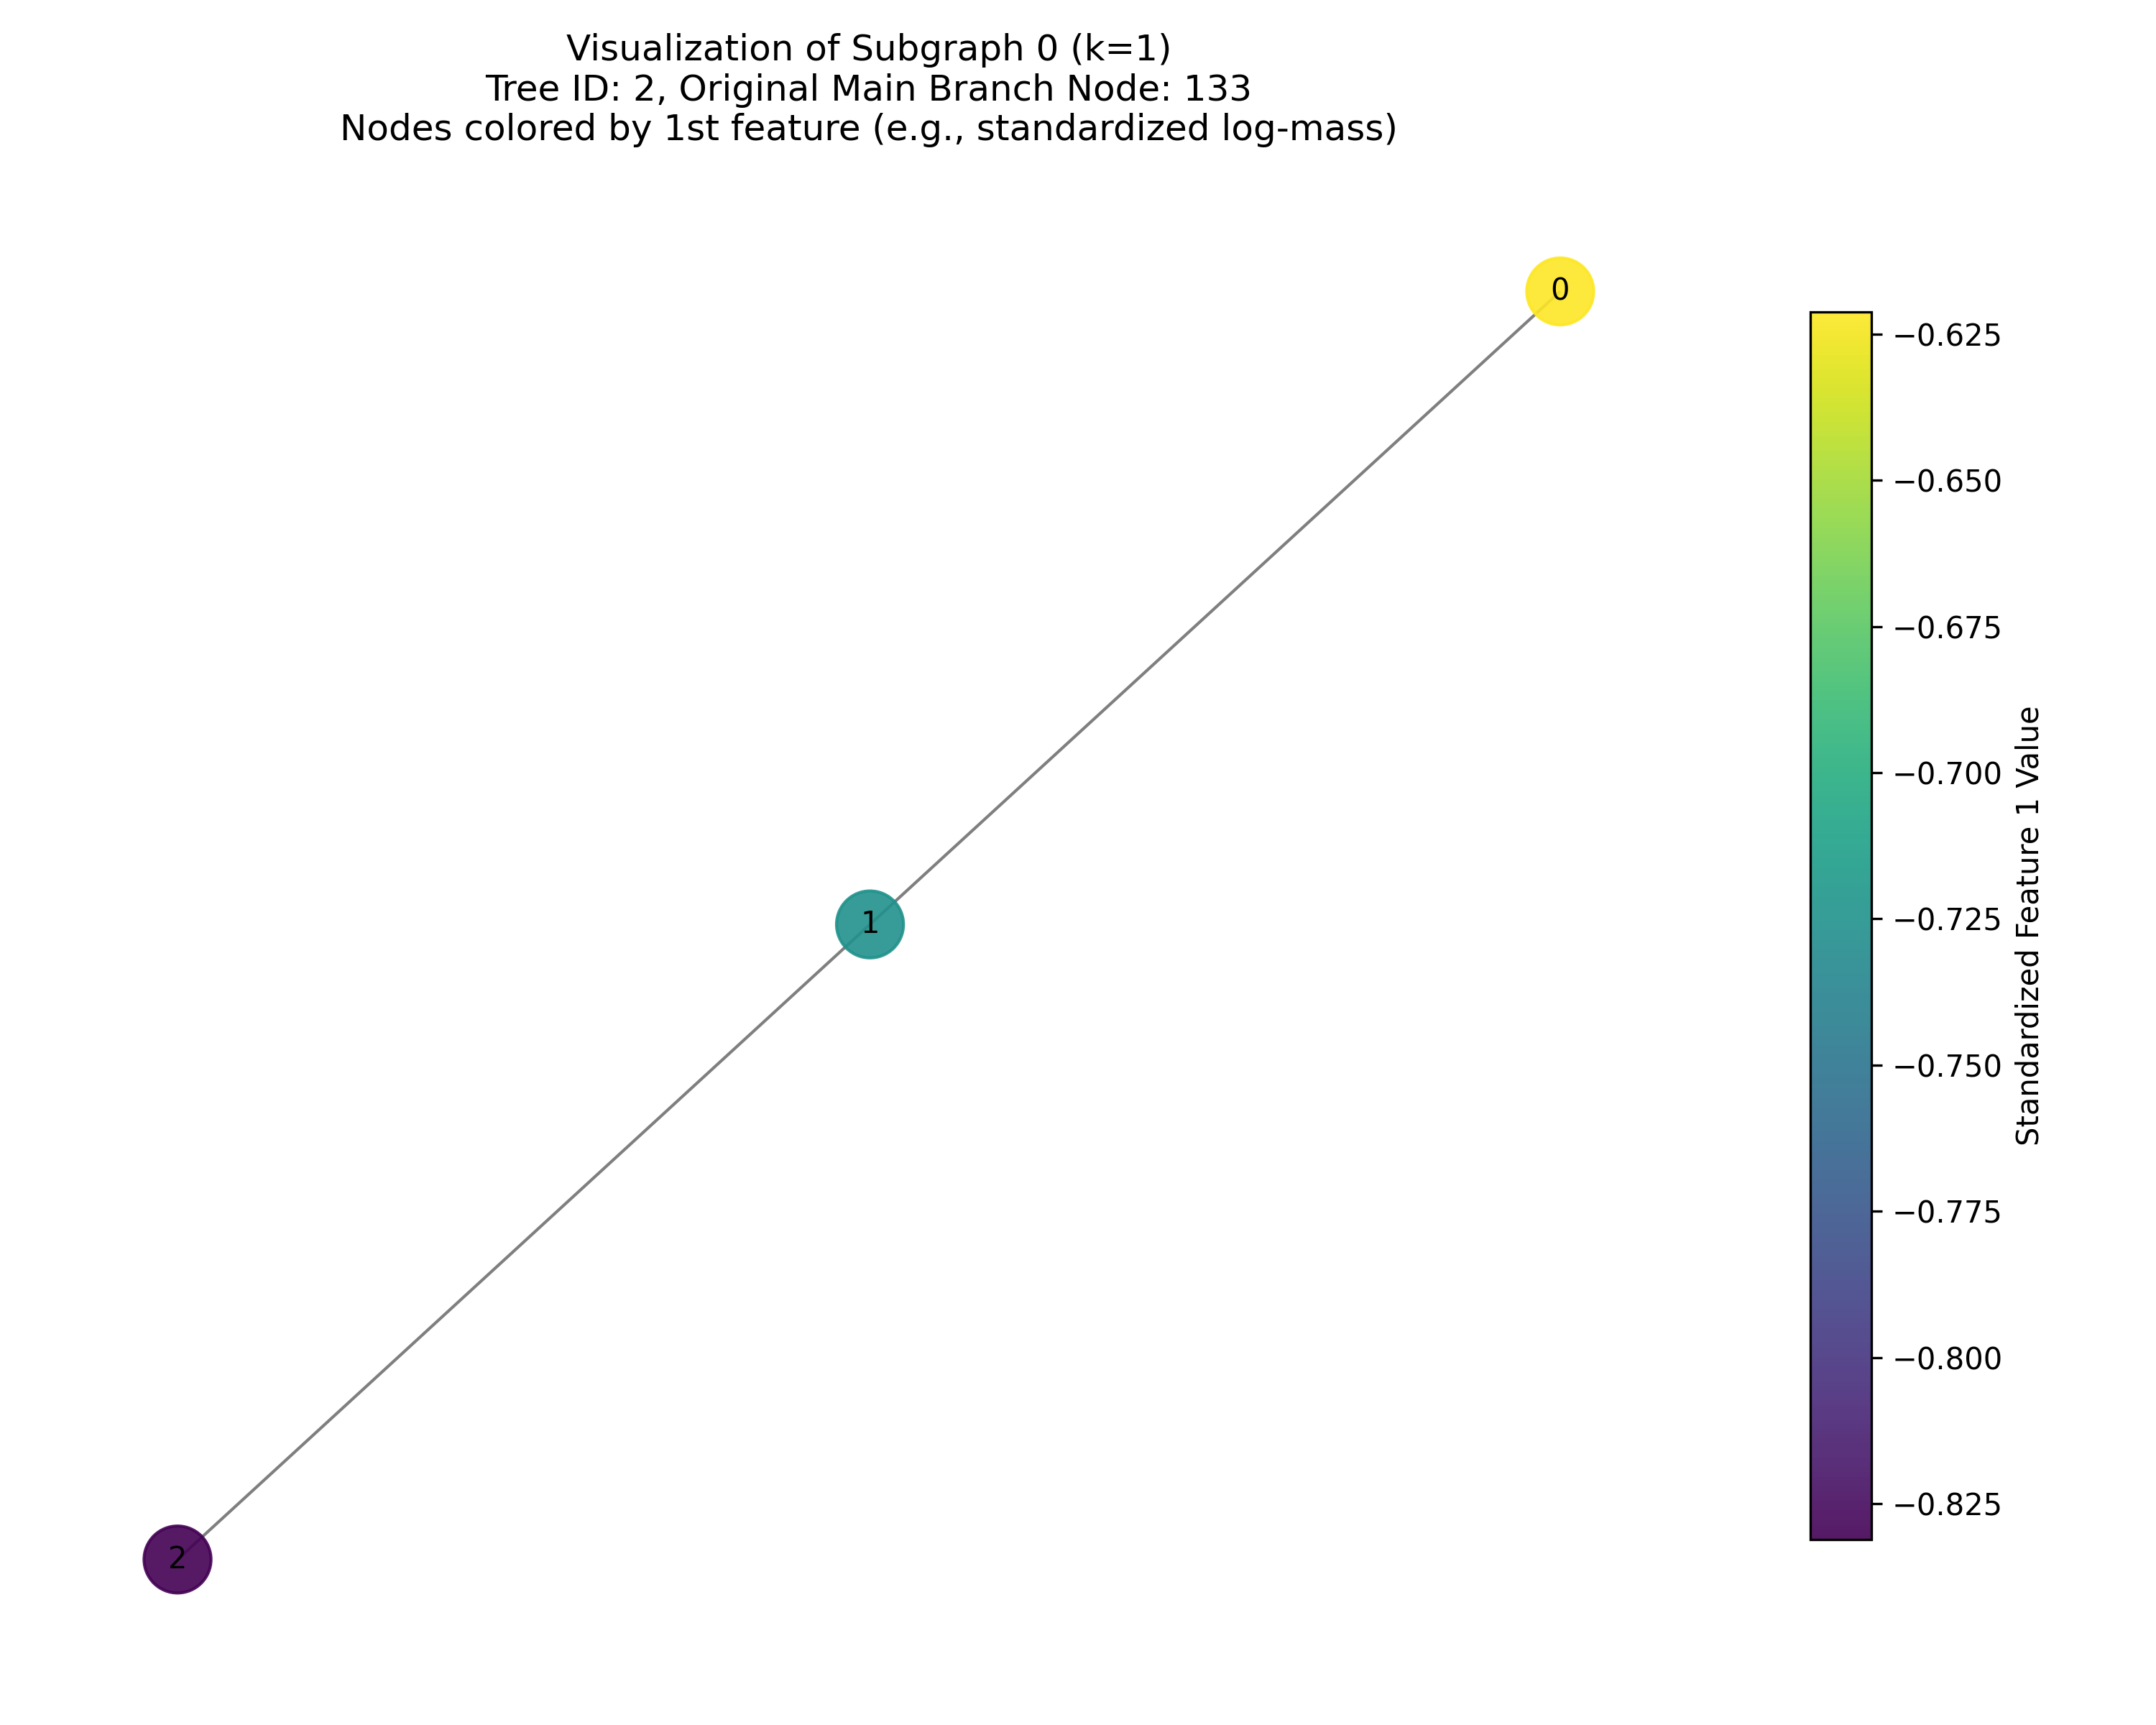
\includegraphics[width=0.5\textwidth]{../input_files/plots/subgraph_vis_k1_idx0_5_20250524-175501.png}
    \caption{Visualization of a sample 1-hop subgraph from a merger tree, with nodes colored by their standardized log-mass. This plot illustrates the local environment around a main branch node, which is then processed by QTT to generate compressed features for predicting final halo mass.
}
    \label{fig:subgraph_vis}
\end{figure}

\subsection{QTT Decomposition and Feature Engineering}

For each of the 5 valid subgraphs, the padded node feature matrix (e.g., shape $[8, 4]$ for $k=1$) was reshaped into a higher-order tensor (e.g., $[2, 2, 2, 4]$ for $k=1$) and decomposed using QTT. Experiments were conducted with QTT ranks of 2 and 3. The QTT cores were then flattened and concatenated to form a single feature vector for each subgraph. For trees with multiple (though in this case, only one per tree) valid main branch subgraphs, these QTT vectors were intended to be aggregated by mean pooling; here, it simply meant taking the QTT vector of the single available subgraph.

The reconstruction Mean Squared Error (MSE) of the QTT decomposition provides an indication of the compression fidelity. For $k=1$ subgraphs, a QTT rank of 2 yielded an average reconstruction MSE of approximately 0.032, while a rank of 3 reduced this to 0.0053. For $k=2$, rank 2 gave an MSE of 0.033, and rank 3 gave 0.016. For $k=3$, rank 2 resulted in an MSE of 0.057, and rank 3 in 0.027. These low MSE values suggest that QTT, even with relatively low ranks, could reconstruct the (padded) subgraph feature matrices with reasonable accuracy, indicating that the compressed QTT features retained substantial information from the local subgraph environments.

\subsection{Regression Performance for Final Halo Mass Prediction}

Random Forest Regressors were trained to predict the first component of the target variable $y$ (representing a final halo mass property at $z=0$), using either baseline aggregated features or the QTT-derived features. Given $N=5$, all evaluations are in-sample.

\subsubsection{Baseline Model}
Baseline features were constructed by taking the mean, maximum, and variance of the four preprocessed node features along the (valid portion of the) main branch for each of the 5 trees. This resulted in a 12-dimensional feature vector per tree.
The baseline model achieved:
\begin{itemize}
    \item Mean Squared Error (MSE): 0.00197
    \item Mean Absolute Error (MAE): 0.0315
    \item R-squared (R²): 0.797
\end{itemize}

\begin{figure}[h!]
    \centering
    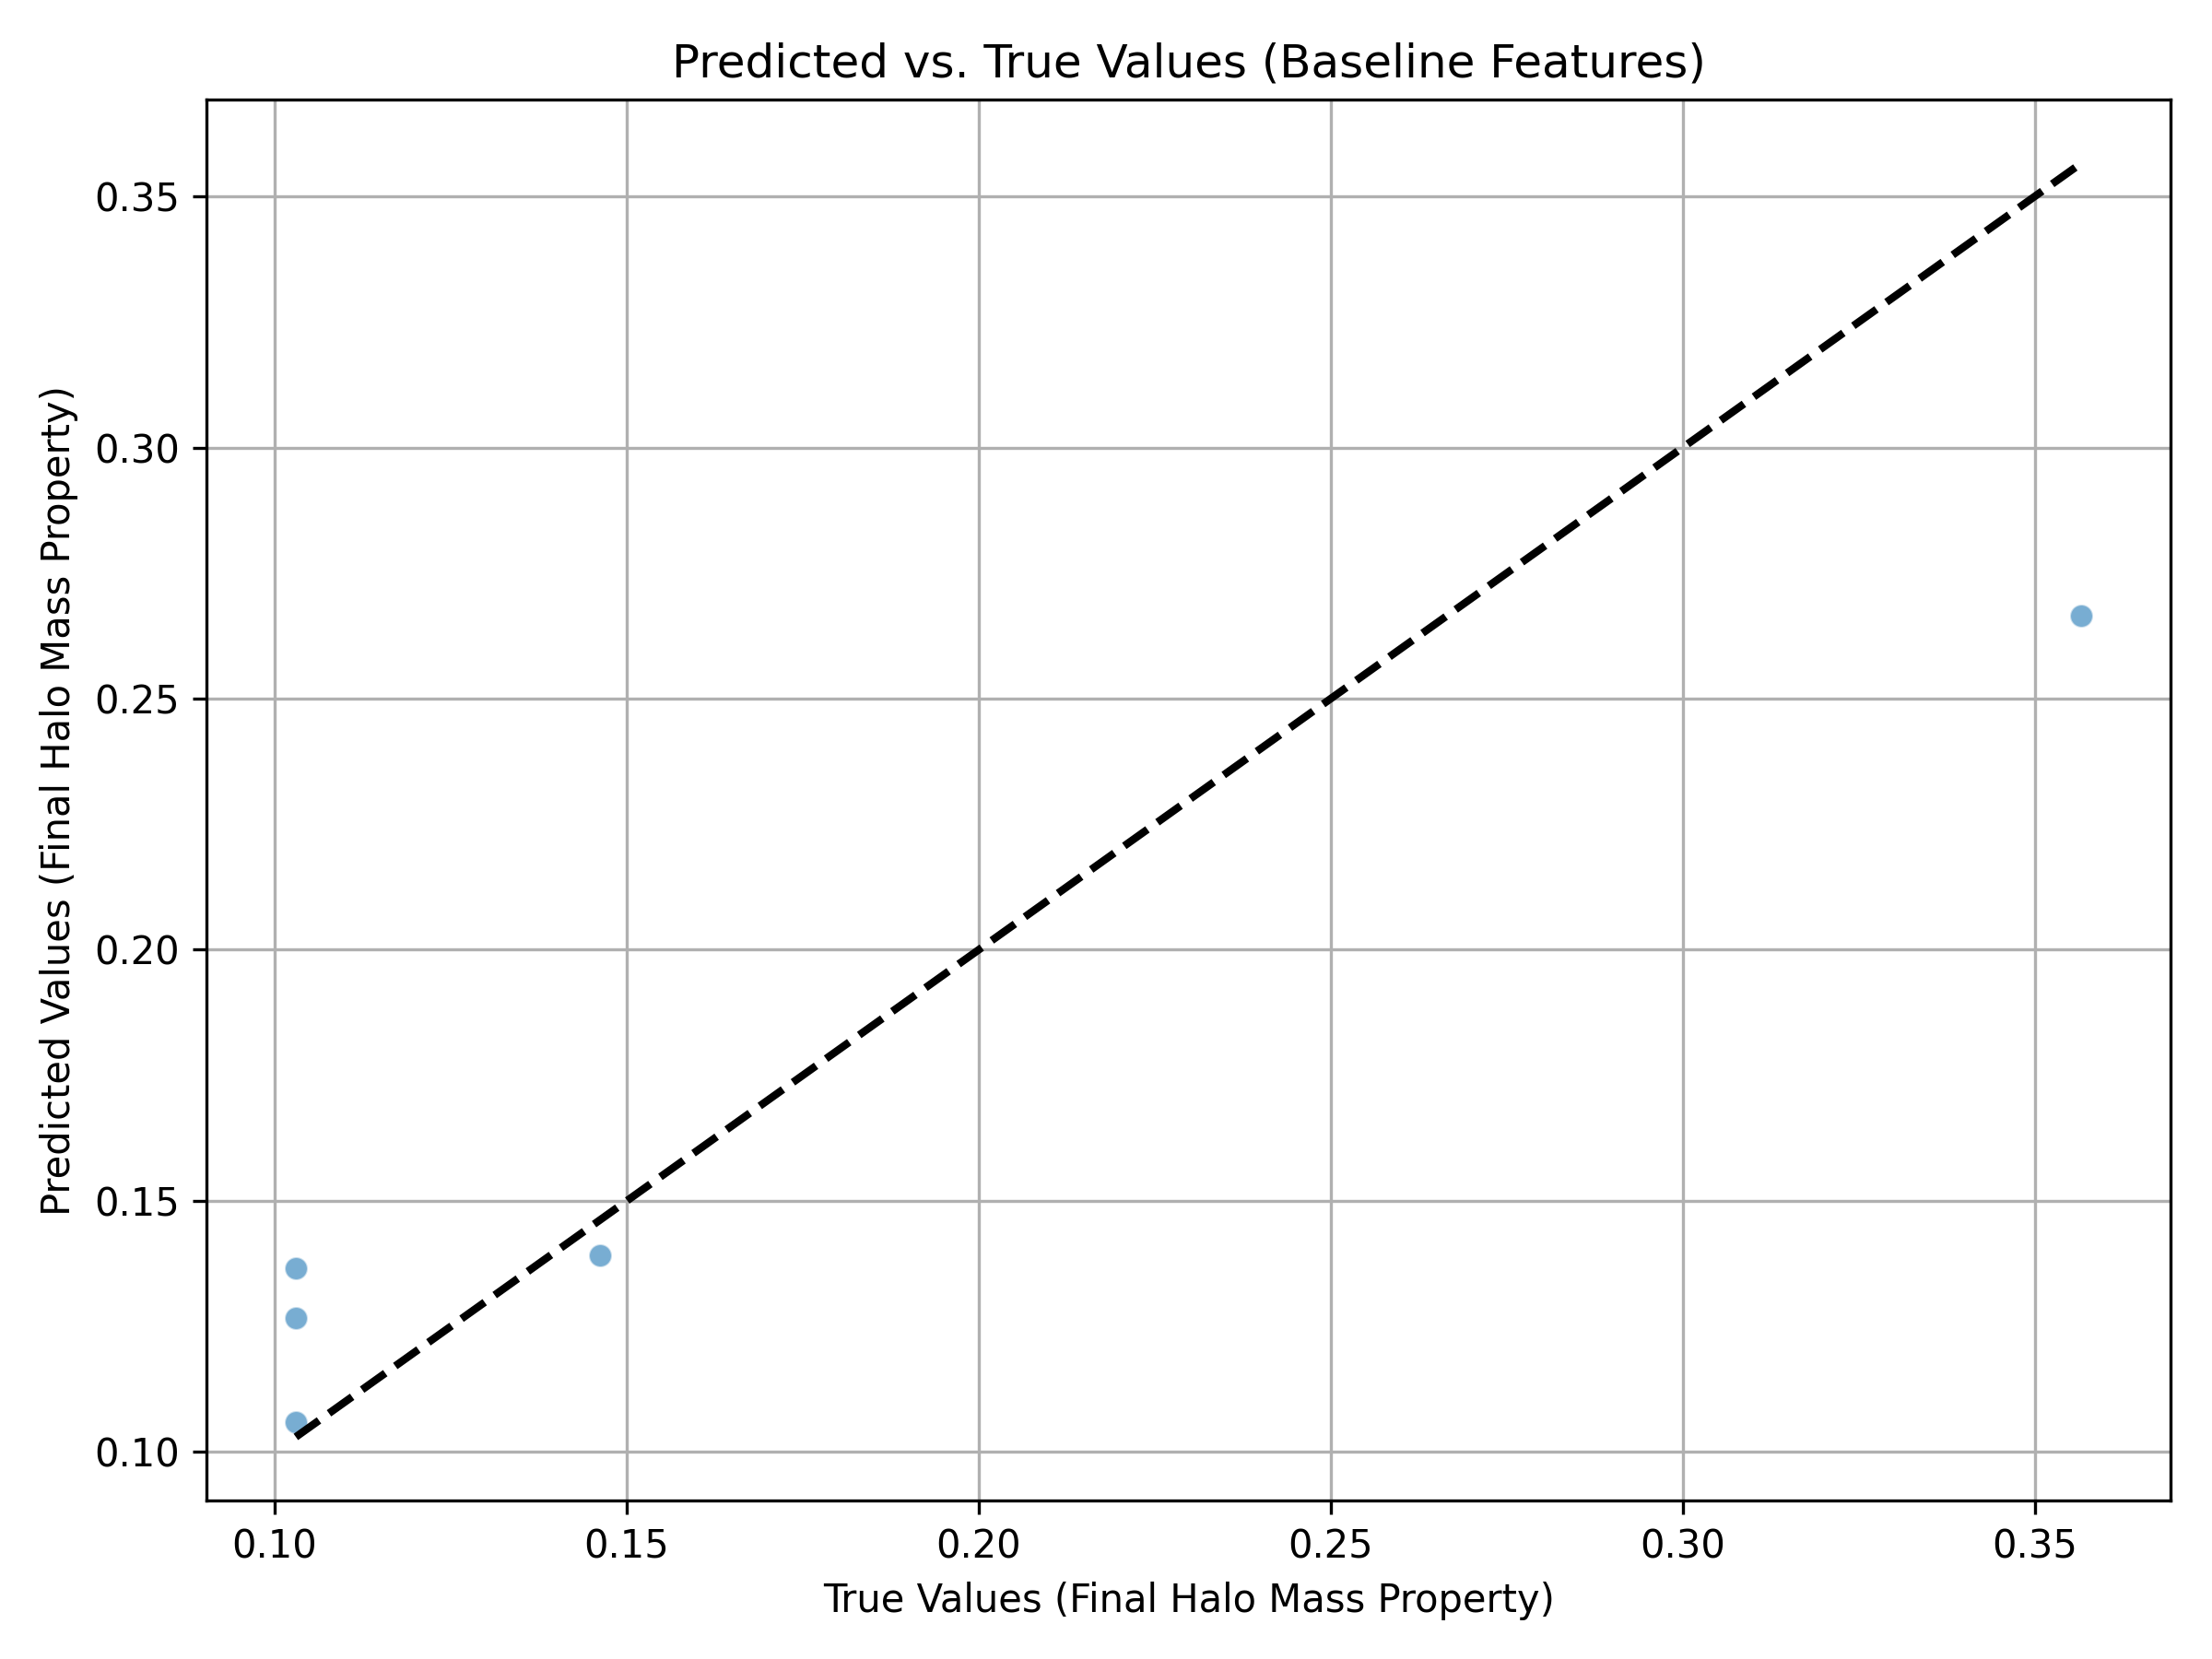
\includegraphics[width=0.5\textwidth]{../input_files/plots/pred_vs_true_baseline_1_20250524-175150.png}
    \caption{Scatter plot of predicted versus true final halo mass values for the baseline model, evaluated on the N=5 trees. The dashed line represents perfect prediction. The clustering of points indicates that the baseline features capture some trend in the data, but due to the small sample size, the high R-squared value should be interpreted with caution.
}
    \label{fig:pred_vs_true_baseline}
\end{figure}

\subsubsection{QTT-based Models}
The performance of QTT-based models varied with $k$ and QTT rank, as detailed in Table 1.

\begin{table}[h!]
    \centering
    \caption{Regression performance of QTT-based models}
    \begin{tabular}{c c c c c}
        \hline
        k & QTT Rank & MSE & MAE & R² \\
        \hline
        1 & 2 & 0.00151 & 0.0261 & 0.845 \\
        1 & 3 & 0.00159 & 0.0276 & 0.836 \\
        2 & 2 & 0.00161 & 0.0279 & 0.834 \\
        2 & 3 & 0.00181 & 0.0291 & 0.813 \\
        3 & 2 & 0.00196 & 0.0348 & 0.798 \\
        3 & 3 & 0.00187 & 0.0341 & 0.808 \\
        \hline
    \end{tabular}
\end{table}

\begin{figure}[h!]
    \centering
    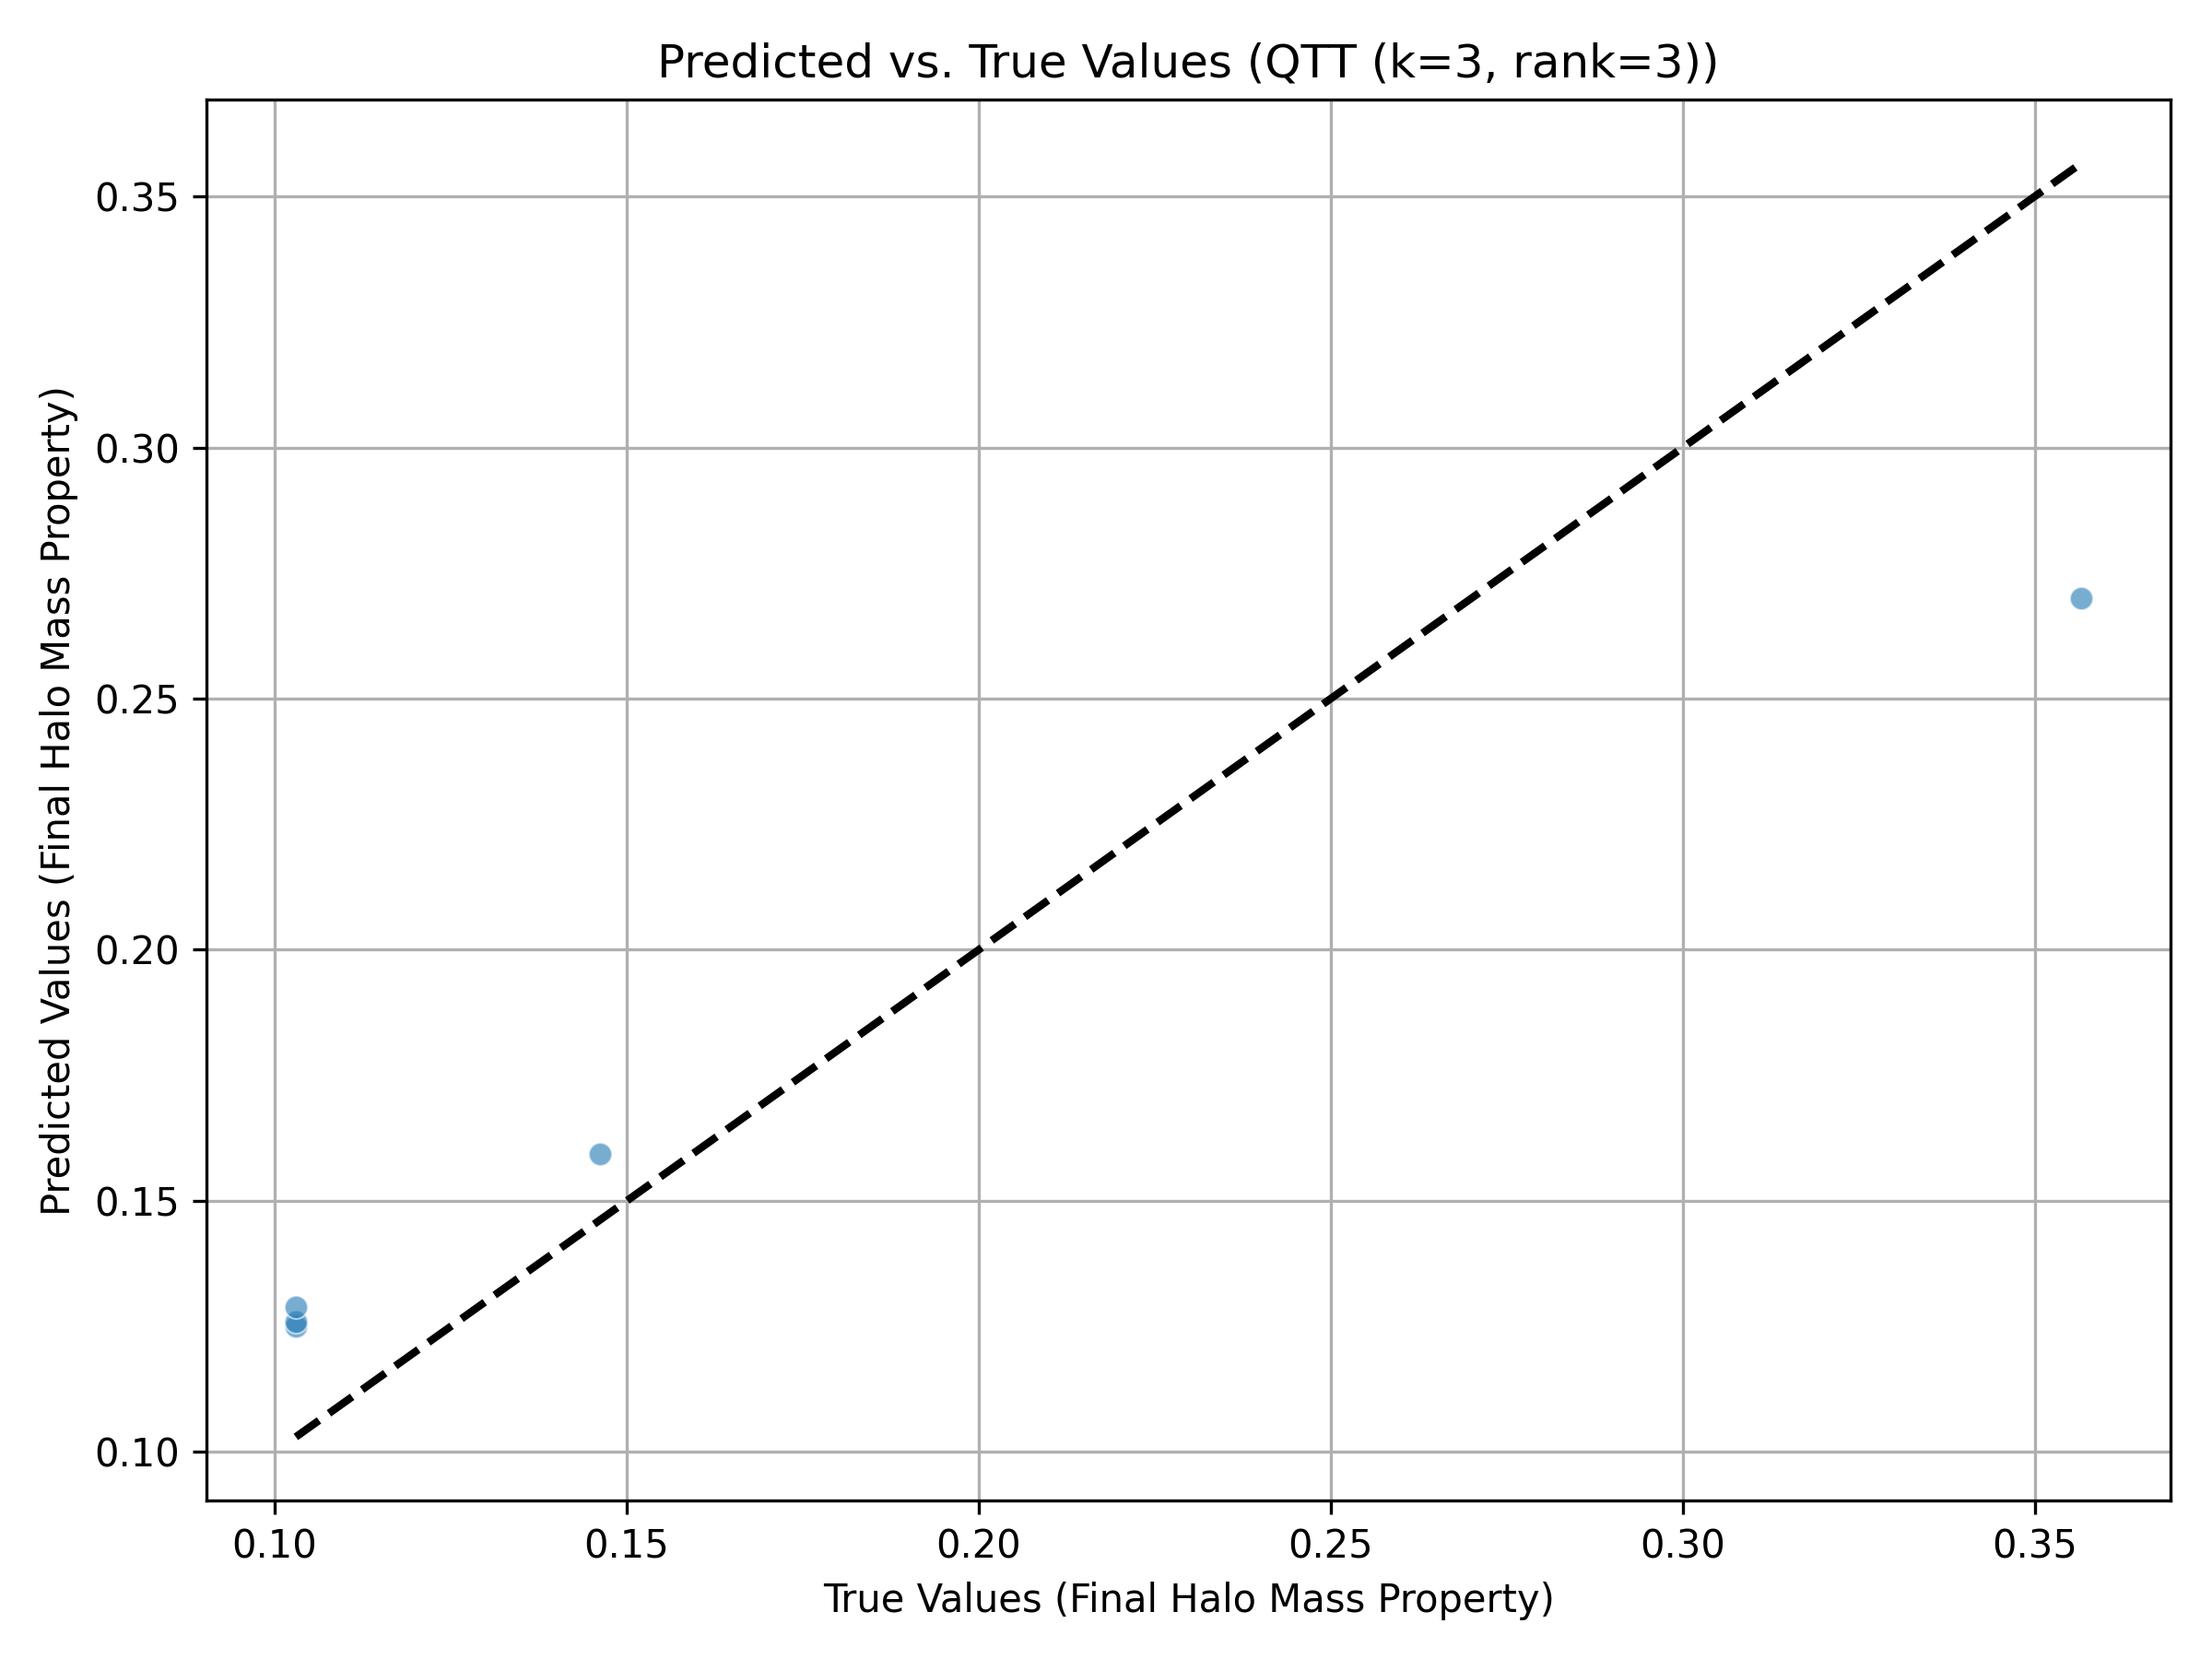
\includegraphics[width=0.5\textwidth]{../input_files/plots/pred_vs_true_qtt_k3_r3_19_20250524-175150.png}
    \caption{Scatter plot of predicted vs. true halo mass values using QTT features (k=3, rank=3) for the N=5 trees, with points lying close to the diagonal indicating good in-sample fit, though the small sample size limits generalizability.
}
    \label{fig:pred_vs_true_qtt}
\end{figure}

\begin{figure}[h!]
    \centering
    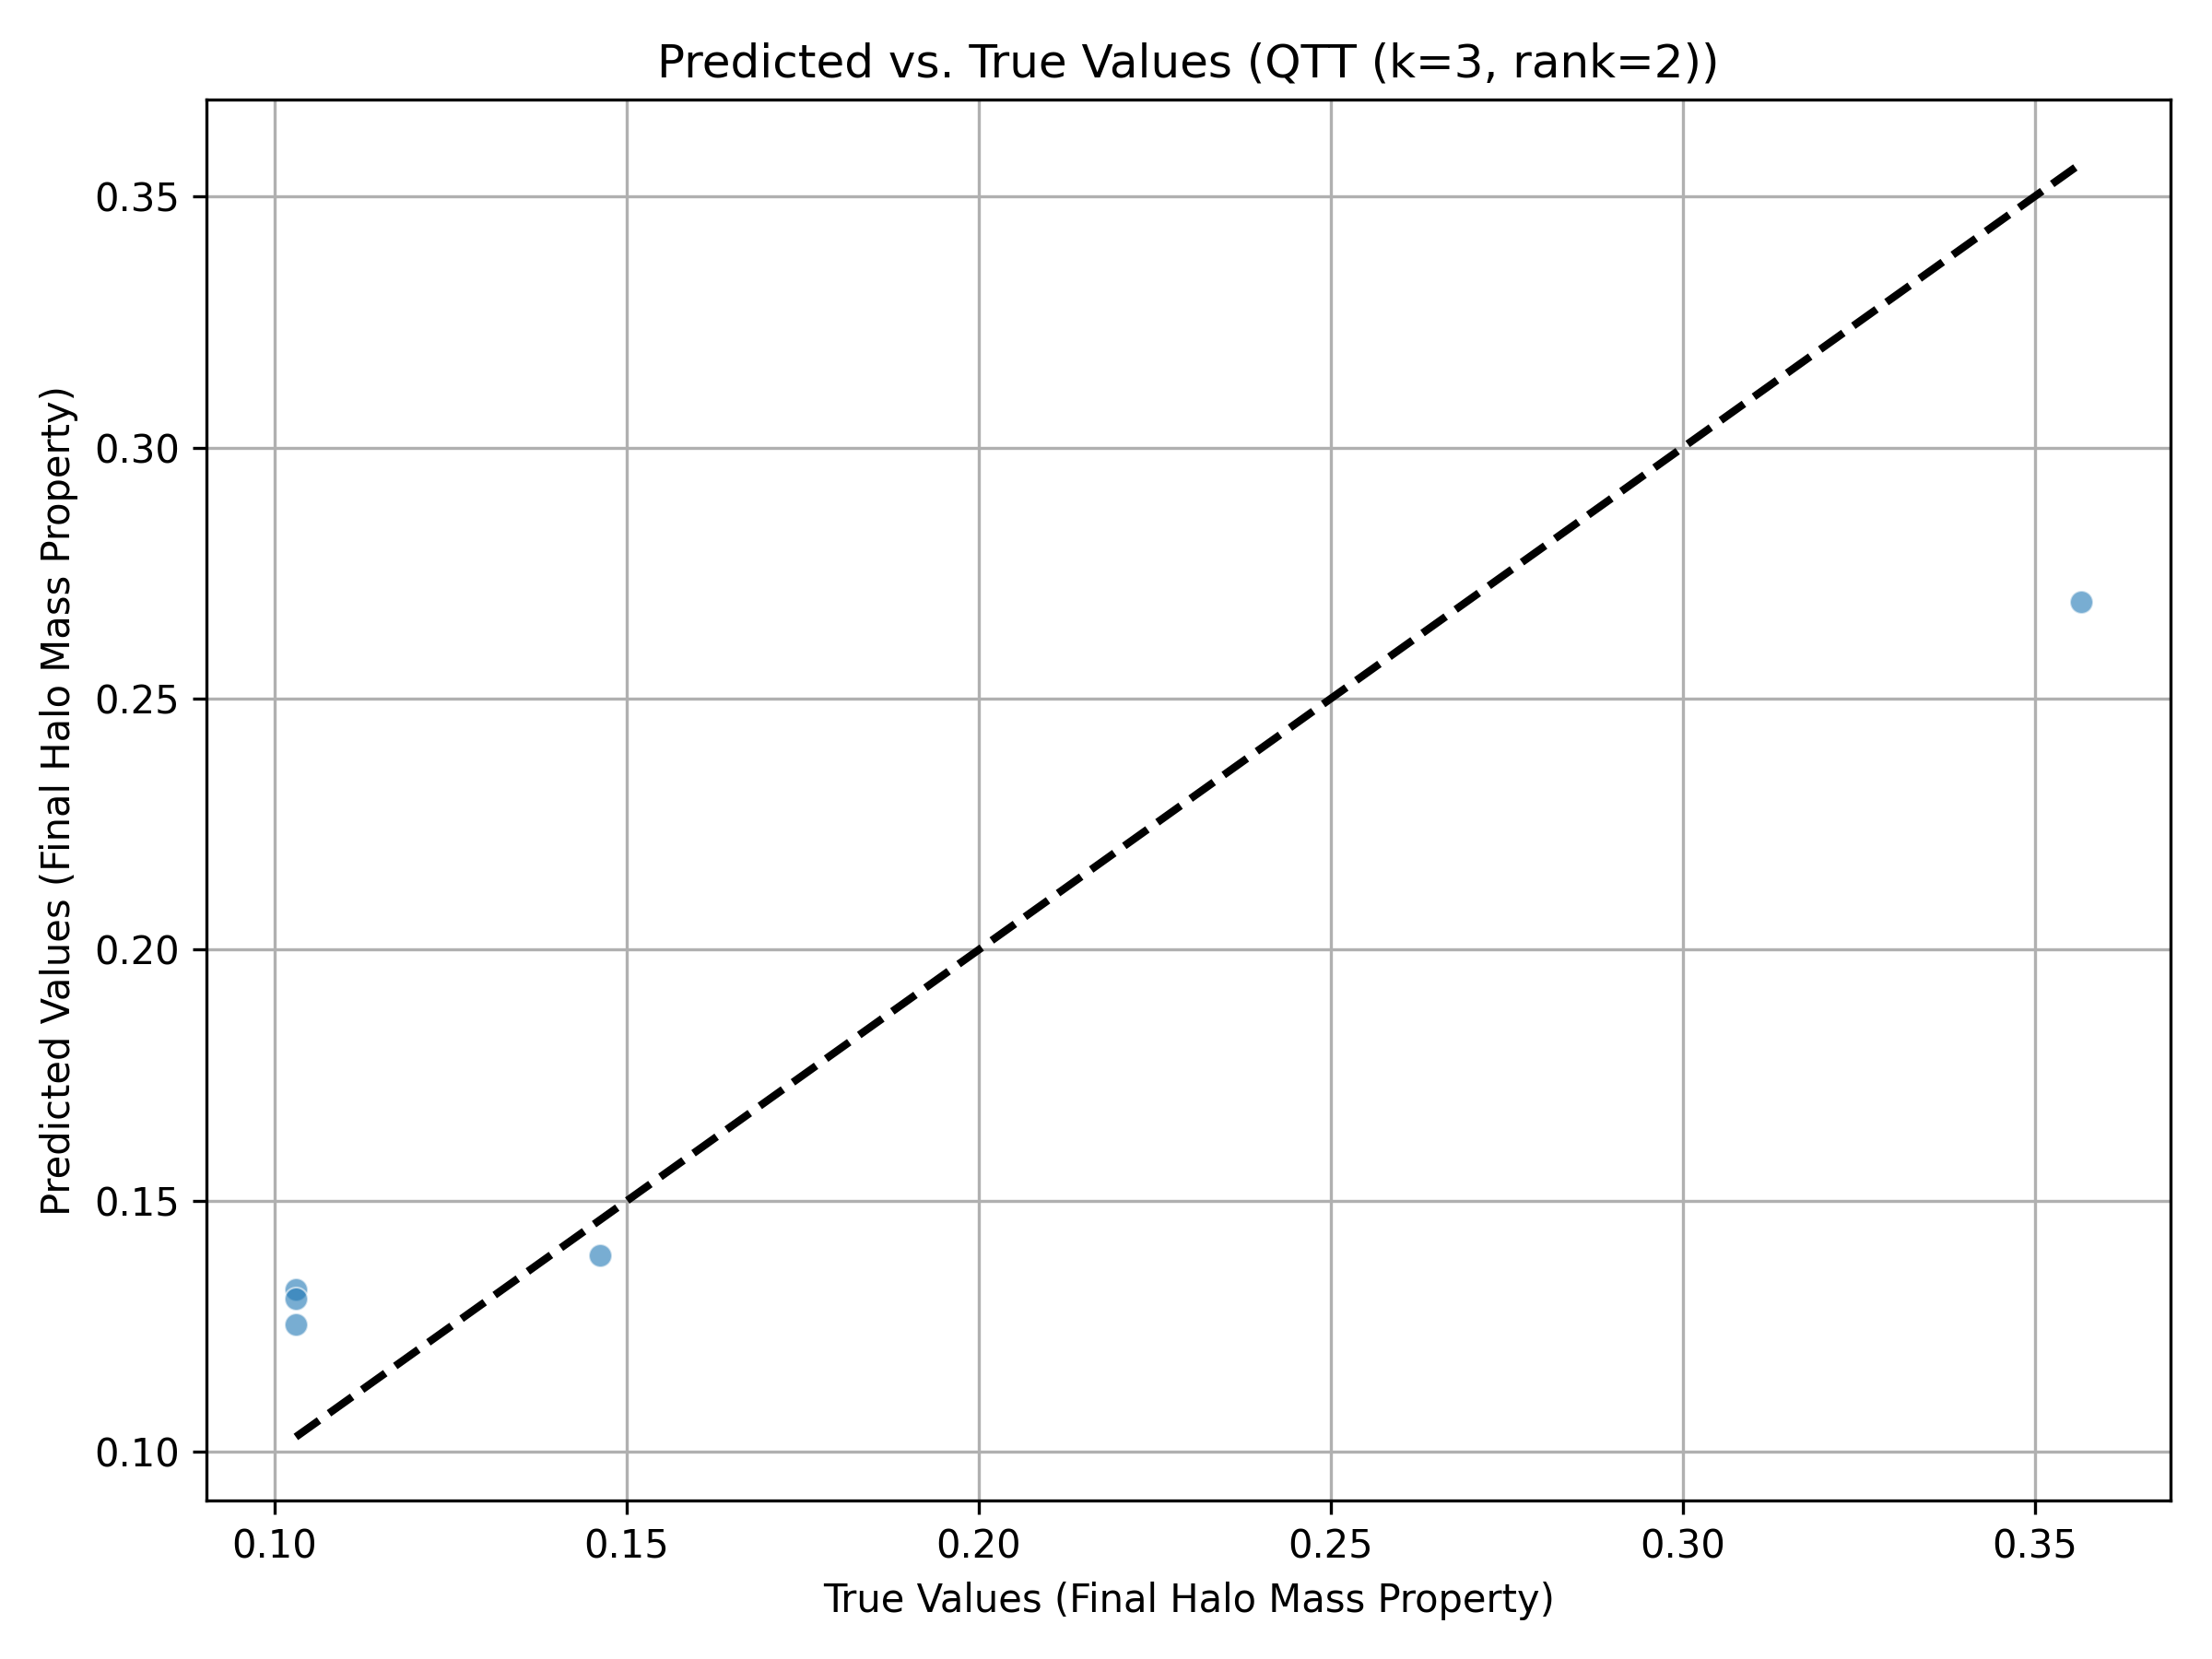
\includegraphics[width=0.5\textwidth]{../input_files/plots/pred_vs_true_qtt_k3_r2_16_20250524-175150.png}
    \caption{Scatter plot of predicted versus true final halo mass values using the QTT model with k=3 and rank=2. The model was trained and evaluated in-sample on N=5 trees, and the dashed line indicates perfect prediction.
}
    \label{fig:pred_vs_true_qtt_k3_r2}
\end{figure}

\begin{figure}[h!]
    \centering
    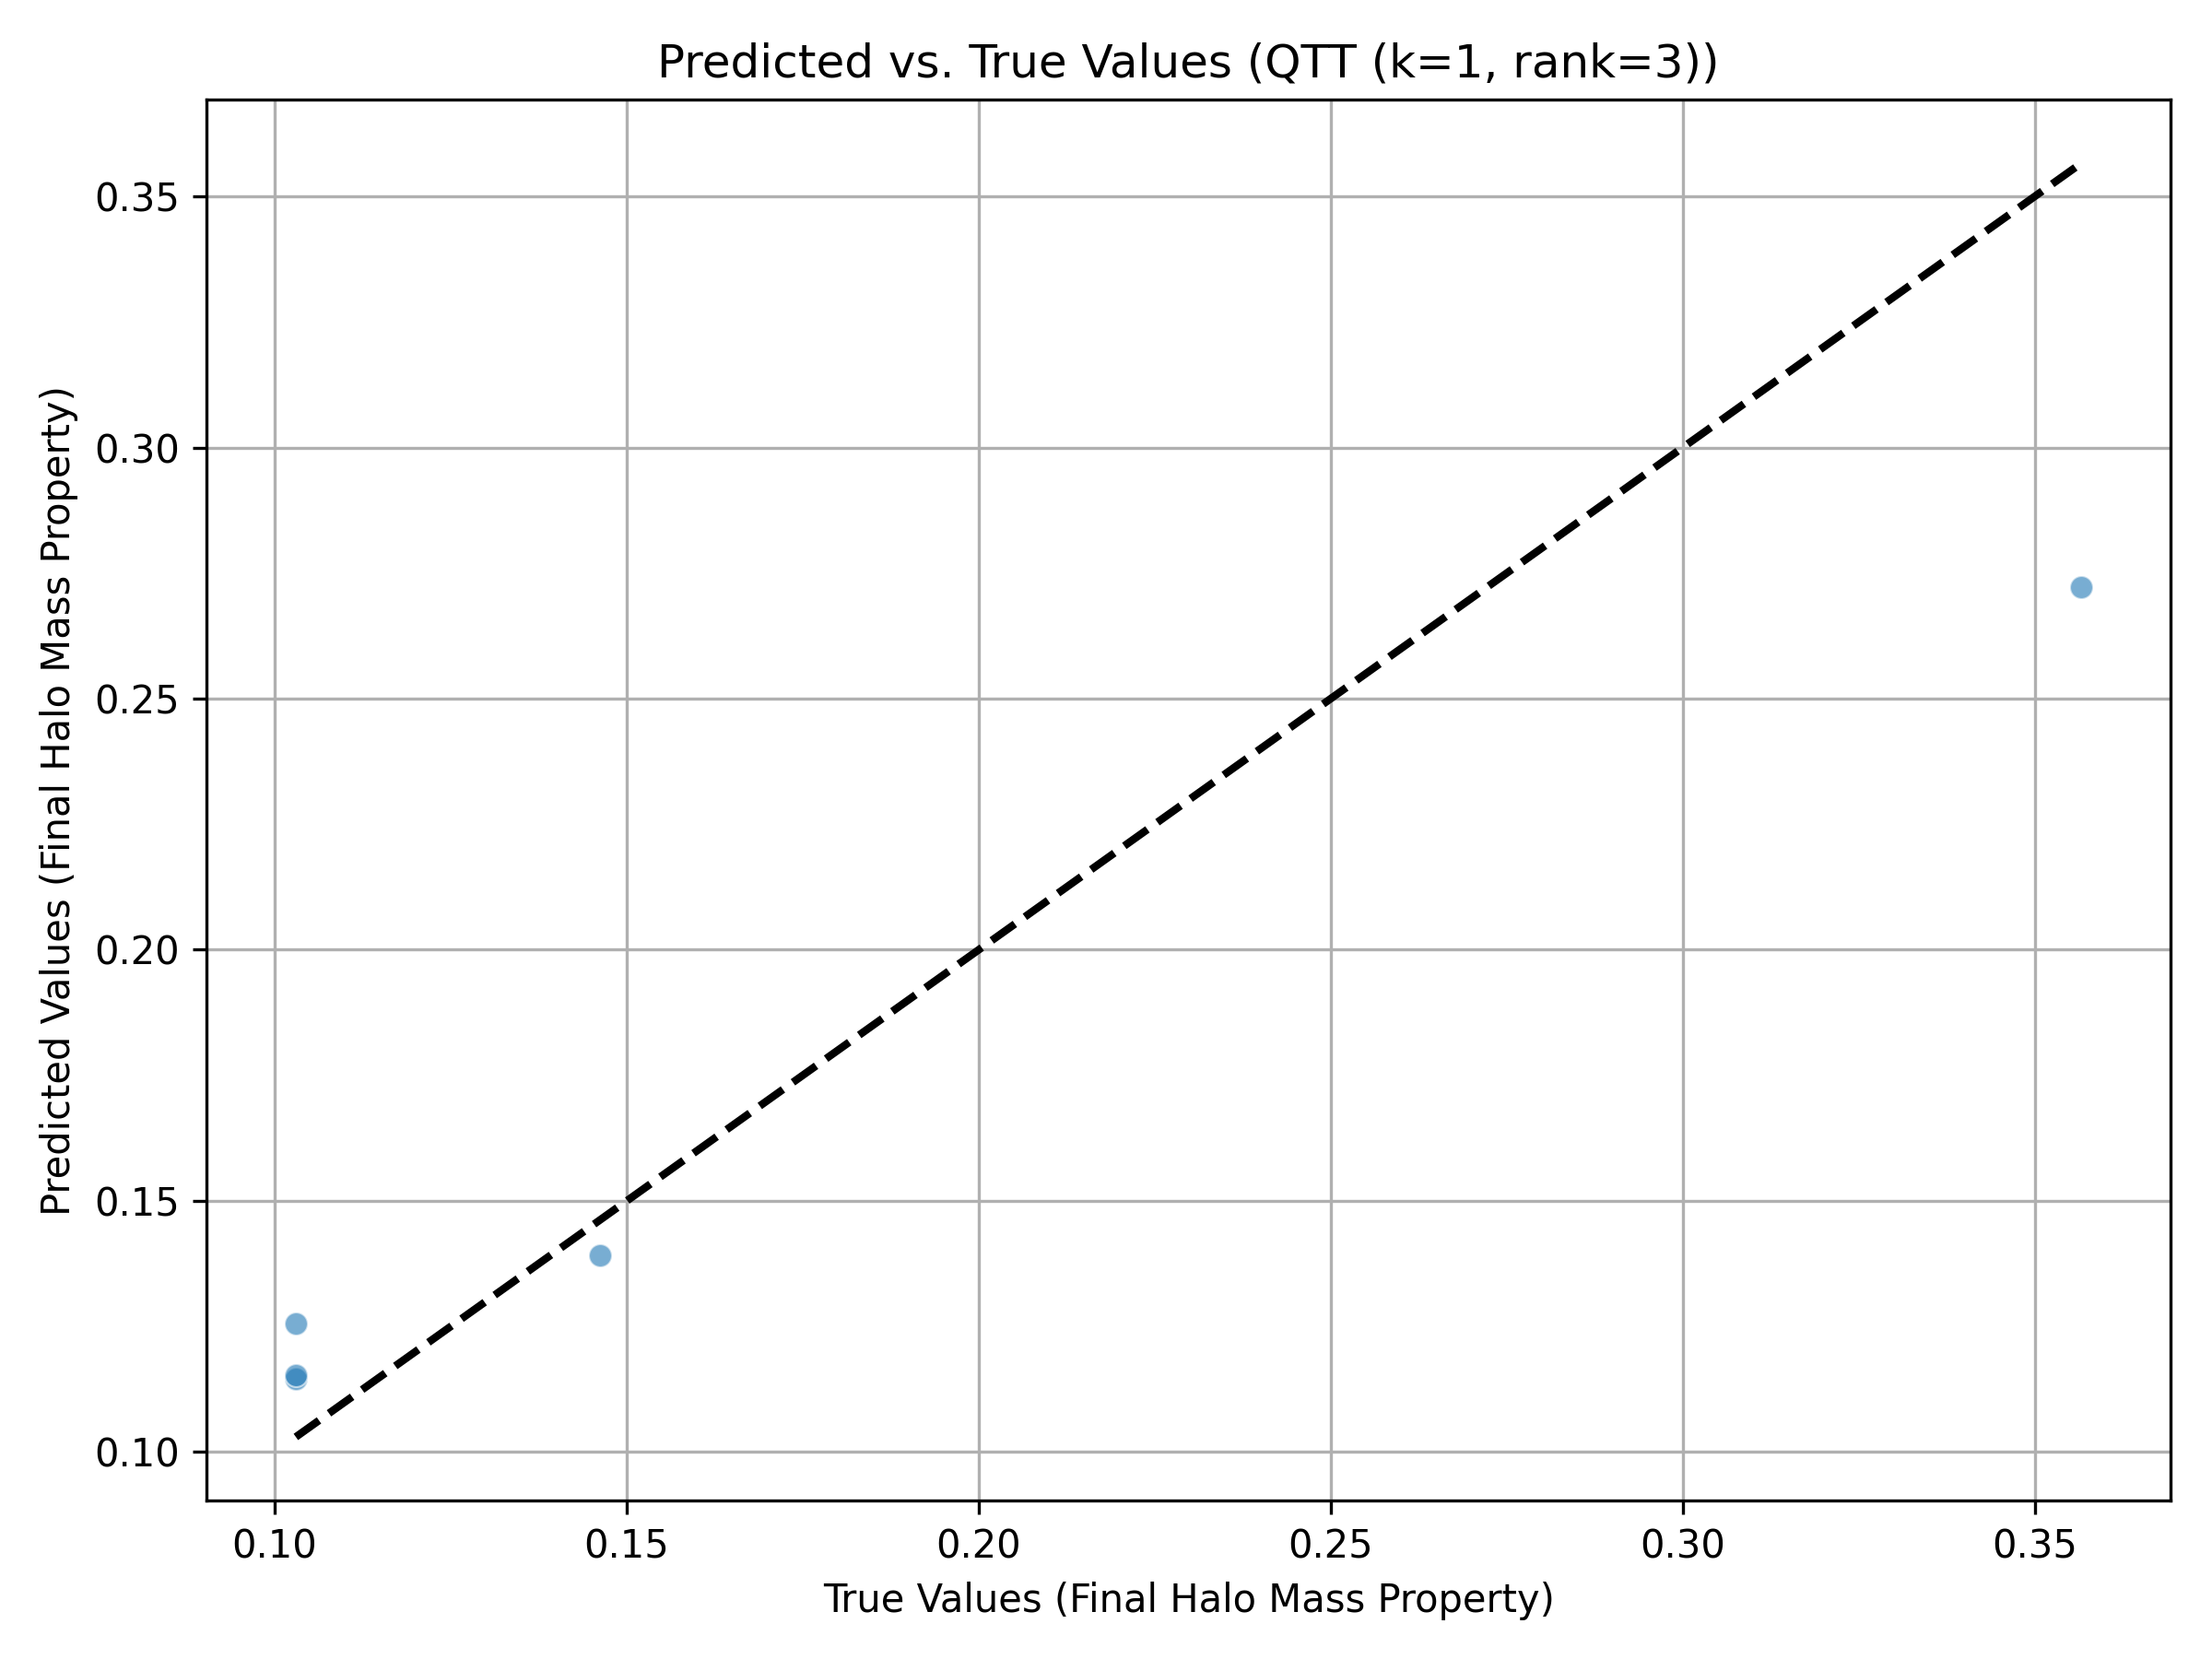
\includegraphics[width=0.5\textwidth]{../input_files/plots/pred_vs_true_qtt_k1_r3_7_20250524-175150.png}
    \caption{Scatter plot of predicted vs. true values for final halo mass using QTT features (k=1, rank=3). The points represent the in-sample predictions for the N=5 trees, and the dashed line indicates perfect prediction. The clustering of points, while seemingly indicative of a relationship, should be interpreted cautiously due to the extremely small sample size.
}
    \label{fig:pred_vs_true_qtt_k1_r3}
\end{figure}

\subsubsection{Comparative Analysis}
Numerically, the QTT model with $k=1$, rank=2 showed the best performance (R²=0.845) among all models, slightly outperforming the baseline (R²=0.797) on this $N=5$ dataset. Other QTT configurations also showed R² values comparable to or slightly better than the baseline.

It is crucial to reiterate that with $N=5$, these differences are not statistically significant and are highly susceptible to the specific characteristics of these five samples. The primary takeaway is that the QTT feature engineering pipeline is functional and can produce features usable by a standard regressor. The observed high R² values, while numerically impressive, should not be interpreted as evidence of a generally superior model without validation on a substantially larger and more representative dataset.

\begin{figure}[h!]
    \centering
    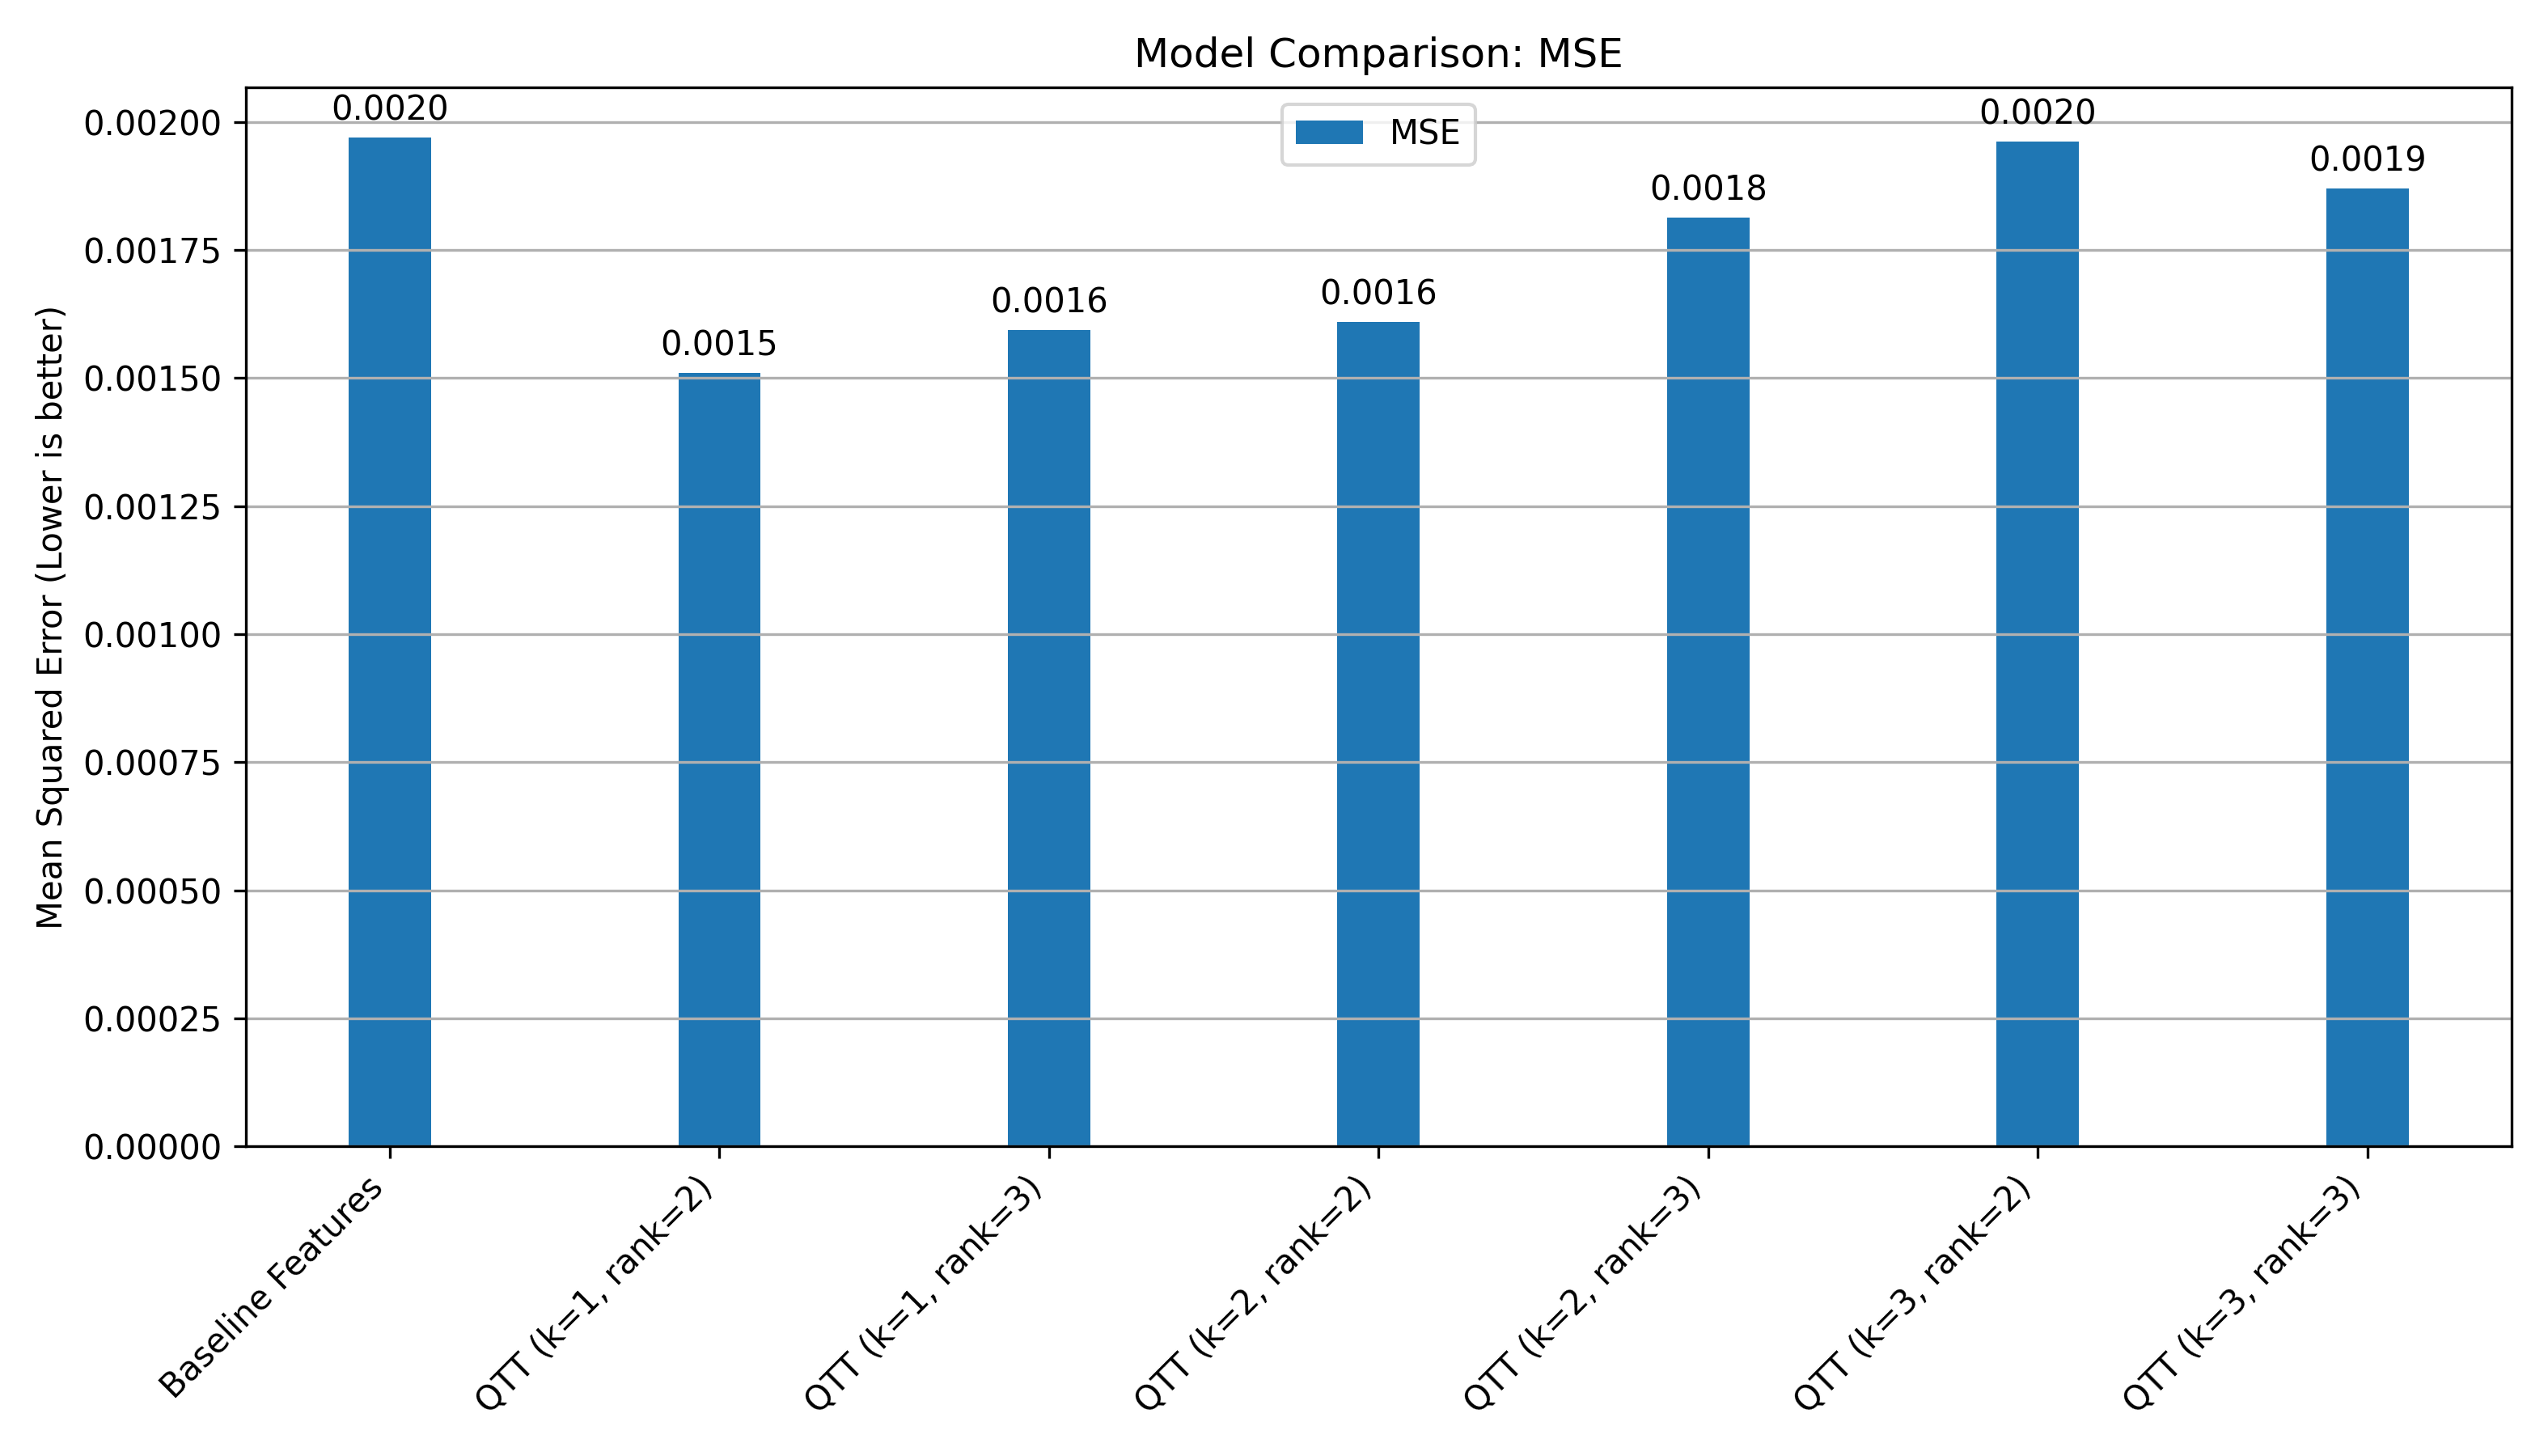
\includegraphics[width=0.5\textwidth]{../input_files/plots/comparison_mse_22_20250524-175150.png}
    \caption{Comparison of Mean Squared Error (MSE) for final halo mass prediction using baseline features and QTT-derived features with varying k-hop neighborhood sizes and QTT ranks. The QTT model with k=1 and rank=2 achieves the lowest MSE on this dataset of N=5 trees.
}
    \label{fig:comparison_mse}
\end{figure}

\begin{figure}[h!]
    \centering
    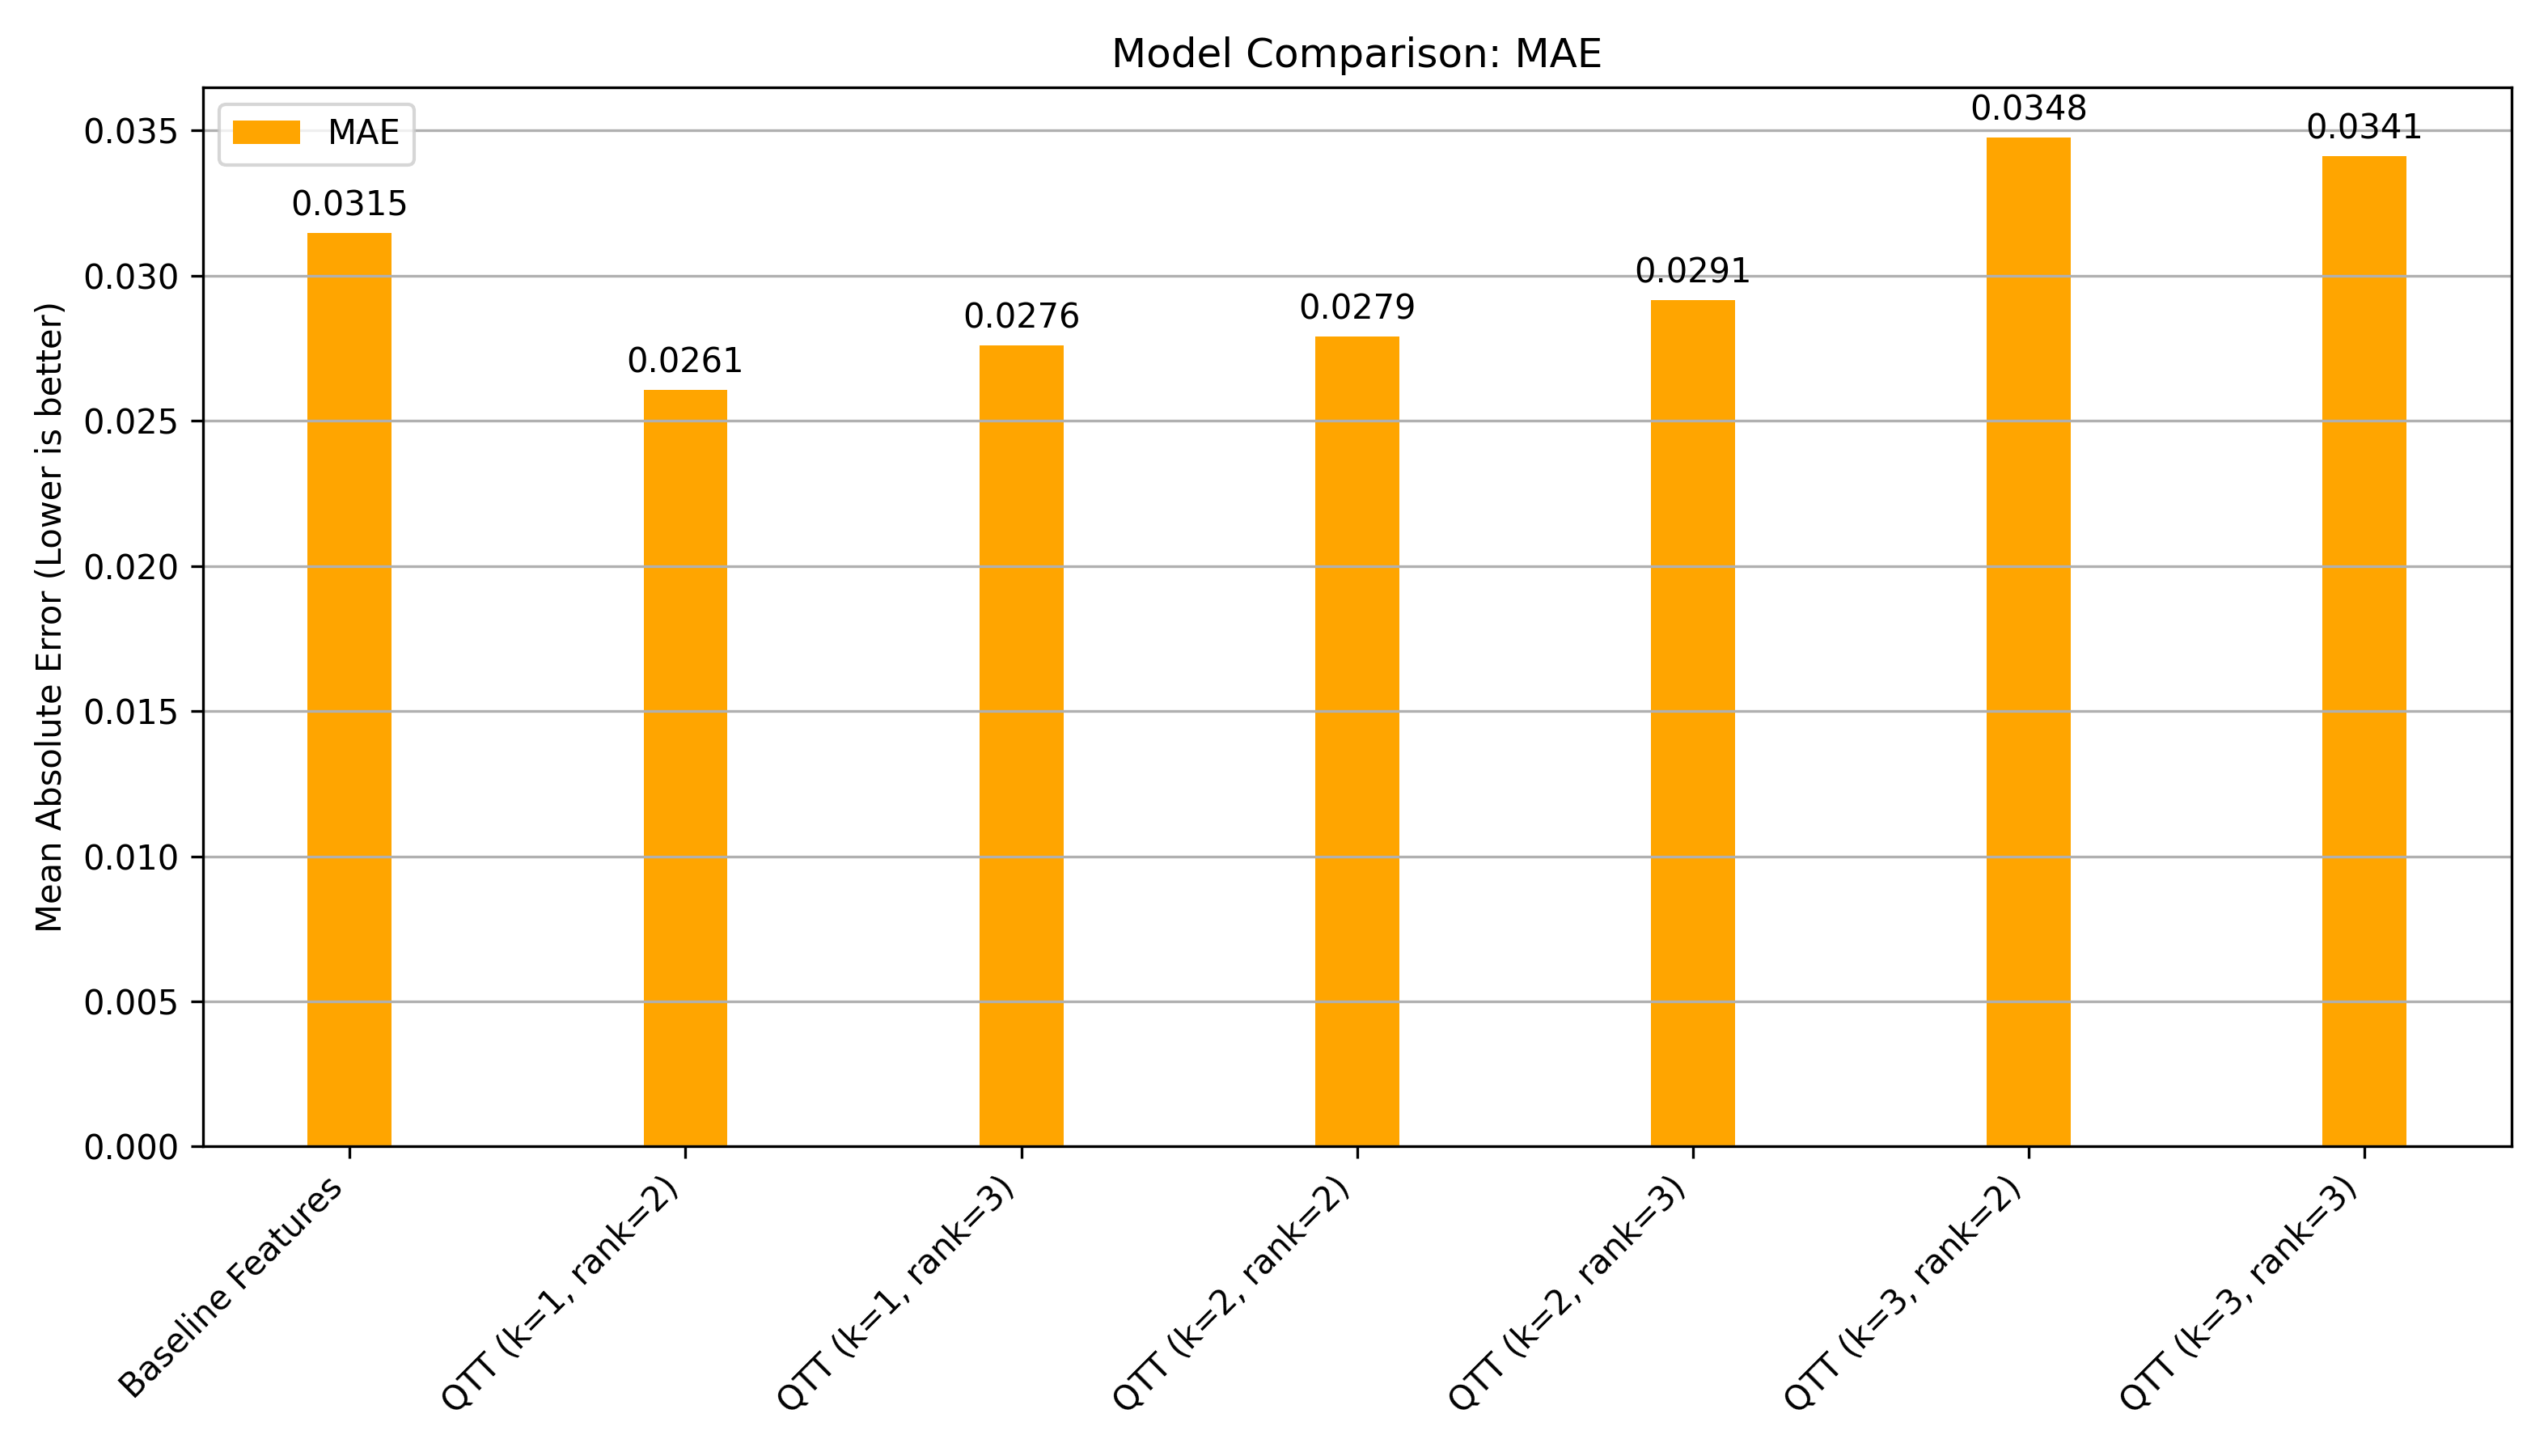
\includegraphics[width=0.5\textwidth]{../input_files/plots/comparison_mae_23_20250524-175150.png}
    \caption{Comparison of Mean Absolute Error (MAE) for final halo mass prediction using baseline features and QTT-derived features with varying k-hop neighborhood sizes and QTT ranks. The results, based on an extremely small sample size (N=5), indicate that QTT features can achieve comparable MAE to the baseline, although these differences are not statistically significant.
}
    \label{fig:comparison_mae}
\end{figure}

\subsection{Feature Space Analysis}

\subsubsection{Feature Distributions}
For the baseline features, the \texttt{*\ensuremath{\_}var} features (variance of mass, concentration, etc., along the main branch) were all zero for the 5 selected trees. This suggests that for these specific trees, either the valid main branch segment consisted of a single node, or the features were constant along the main branch segment. This is another artifact of the extremely small and potentially unrepresentative sample. The \texttt{*\ensuremath{\_}mean} and \texttt{*\ensuremath{\_}max} features showed some variation.

The QTT features, being components of compressed tensor cores, exhibit distributions that are not directly interpretable in terms of physical properties.

\begin{figure}[h!]
    \centering
    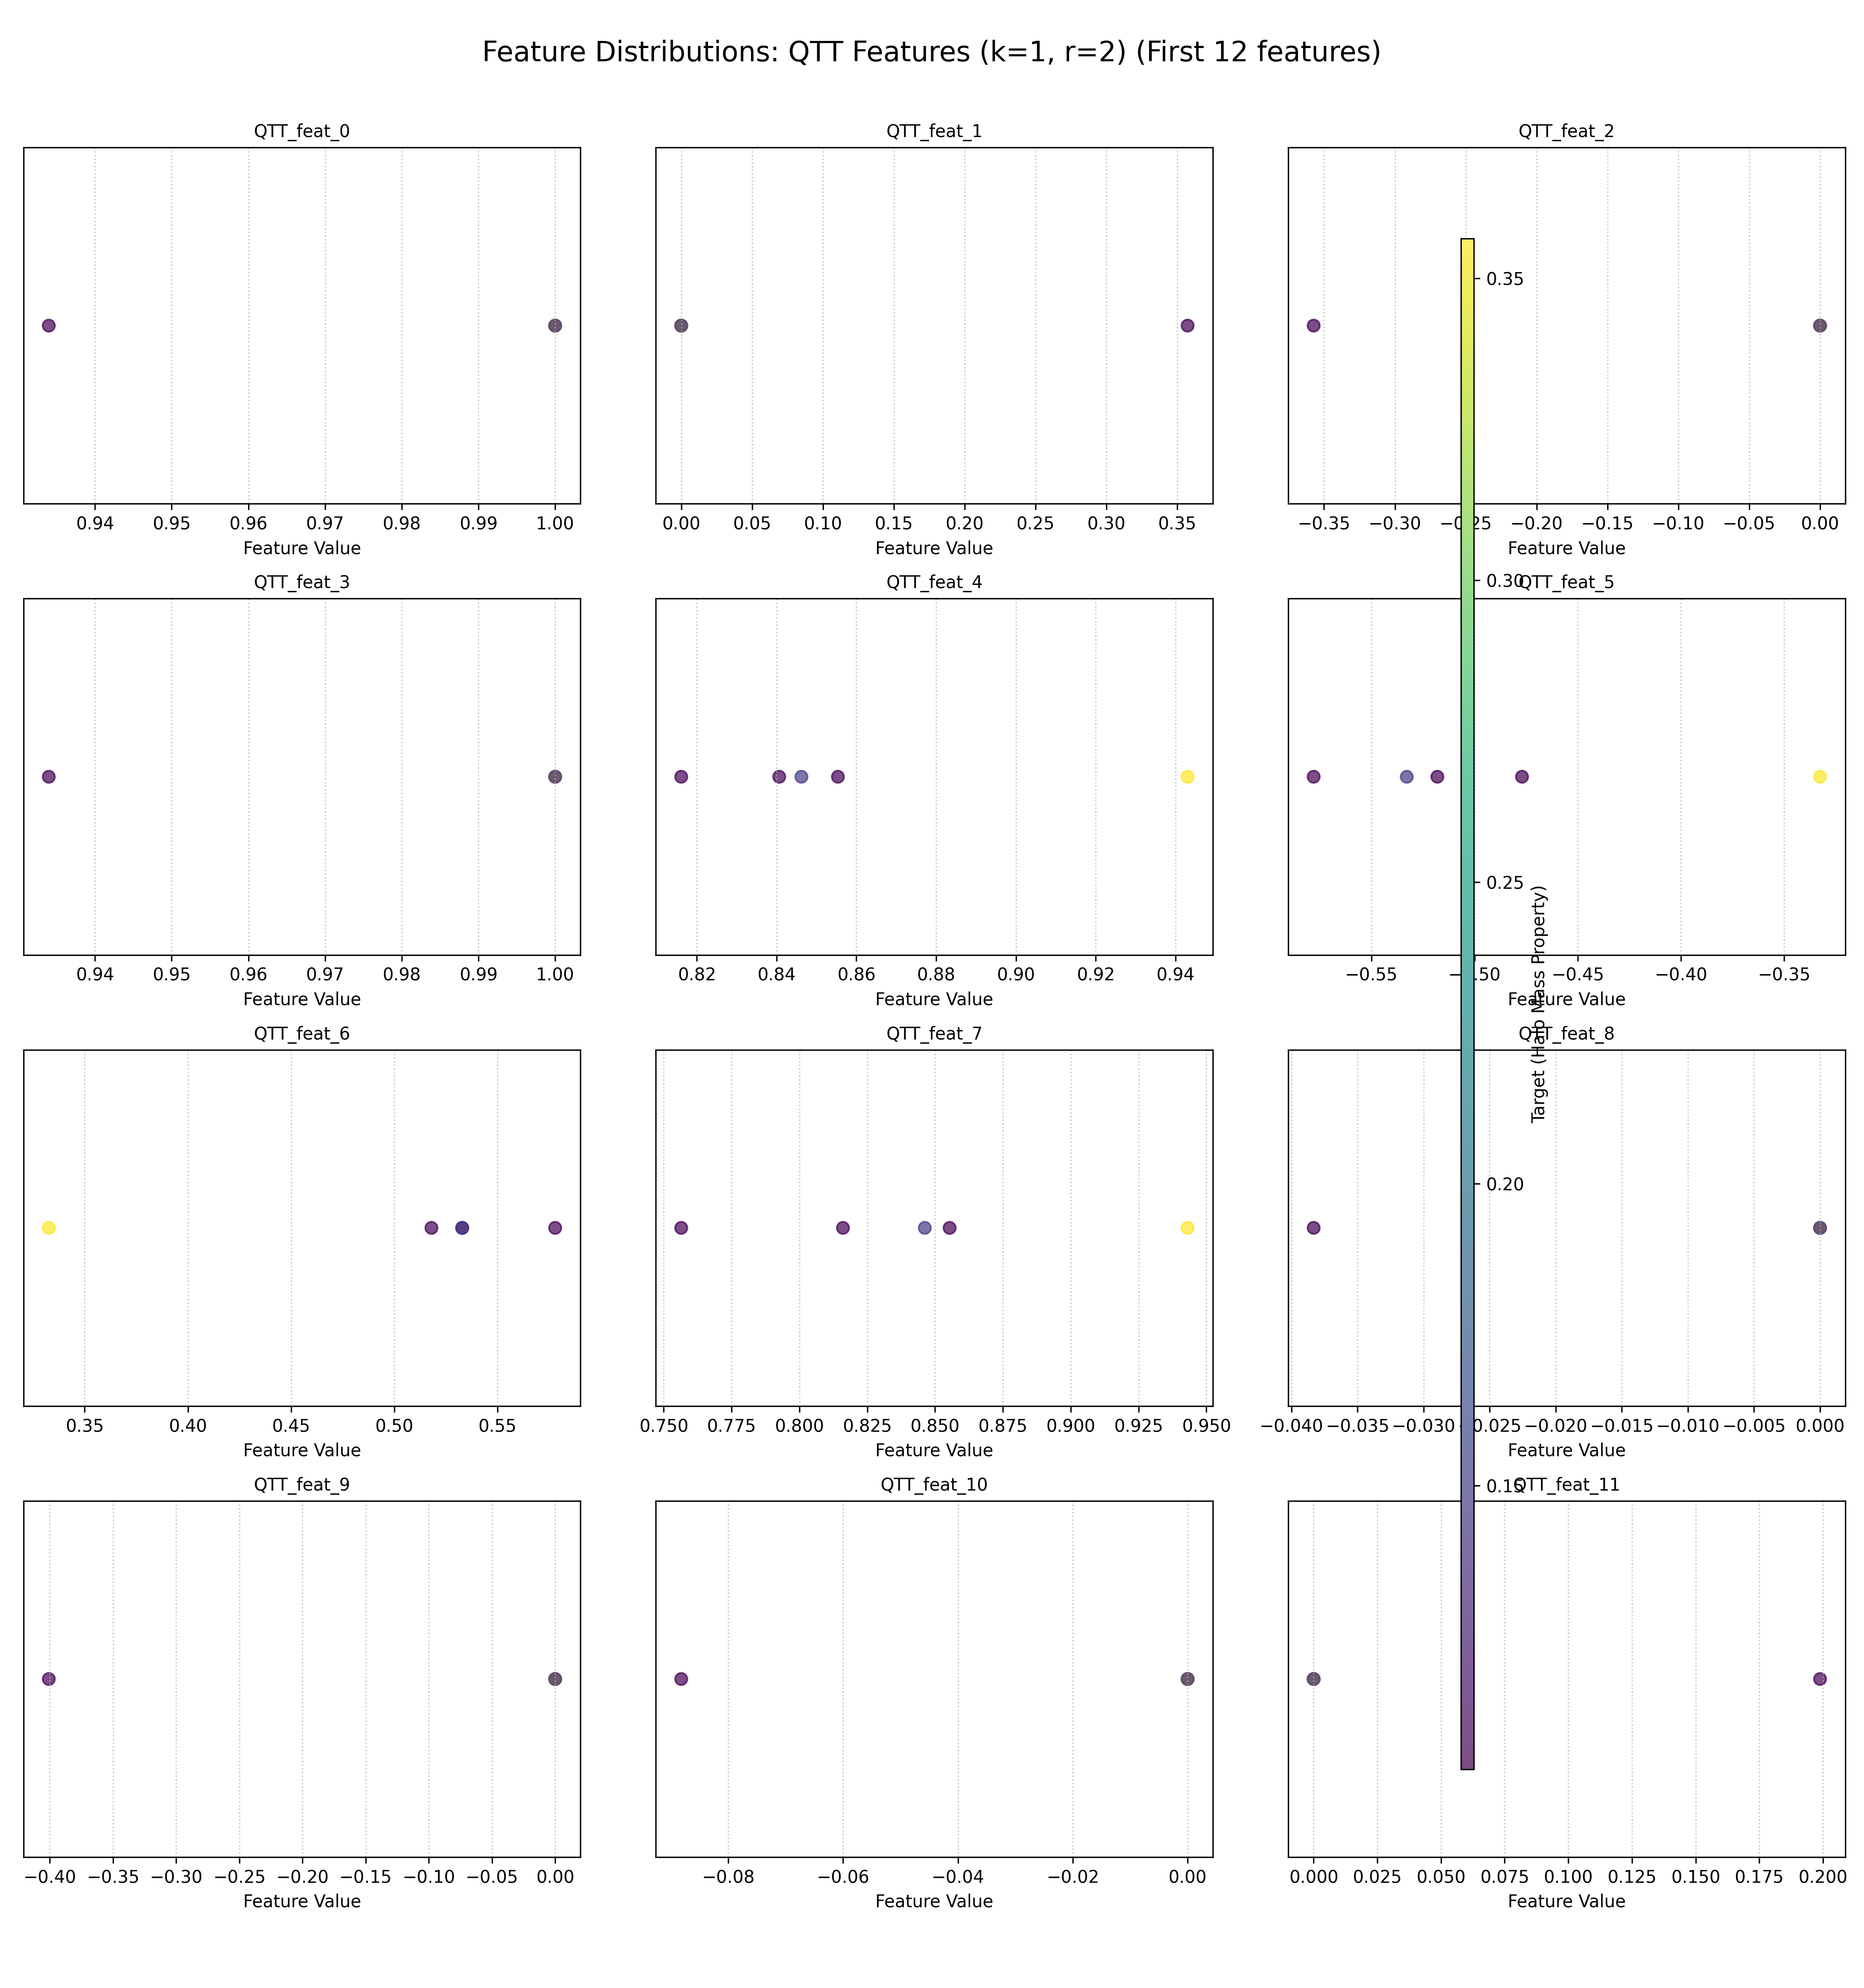
\includegraphics[width=0.5\textwidth]{../input_files/plots/feature_dist_qtt_features_(k=1,_r=2)_2_20250524-175501.png}
    \caption{Distributions of the first 12 QTT features (k=1, rank=2) for the N=5 trees, colored by the target halo mass property. The abstract nature of these features makes direct physical interpretation difficult, but the model assigns varying importances to them for the prediction task.
}
    \label{fig:feature_dist_qtt}
\end{figure}

\subsubsection{Dimensionality Reduction (PCA)}
For the baseline features, the first two principal components explained approximately 75.7\% and 23.6\% of the variance, respectively (total $\sim$99.3\%). For the QTT features ($k=1$, rank=2), the first two components explained about 71.3\% and 24.0\% of the variance (total $\sim$95.3\%). The high cumulative explained variance in both cases suggests that much of the feature variability within this tiny sample can be captured in a low-dimensional space.

\subsubsection{Feature Importances}
For the $N=5$ sample, baseline features like \texttt{mass\ensuremath{\_}mean}, \texttt{vmax\ensuremath{\_}mean}, \texttt{concentration\ensuremath{\_}mean}, and their \texttt{\ensuremath{\_}max} counterparts showed non-zero importance. As noted, \texttt{*\ensuremath{\_}var} features had zero importance because their values were zero.

The QTT feature importance plots show a distribution of importances across the abstract QTT features. For $k=1$, rank=2 (28 features), several features contributed to the prediction. The interpretation of individual QTT feature importances is challenging due to their abstract nature. However, the fact that the model assigns varying importances suggests that different components of the compressed QTT representation contribute differently to the predictive task.

\begin{figure}[h!]
    \centering
    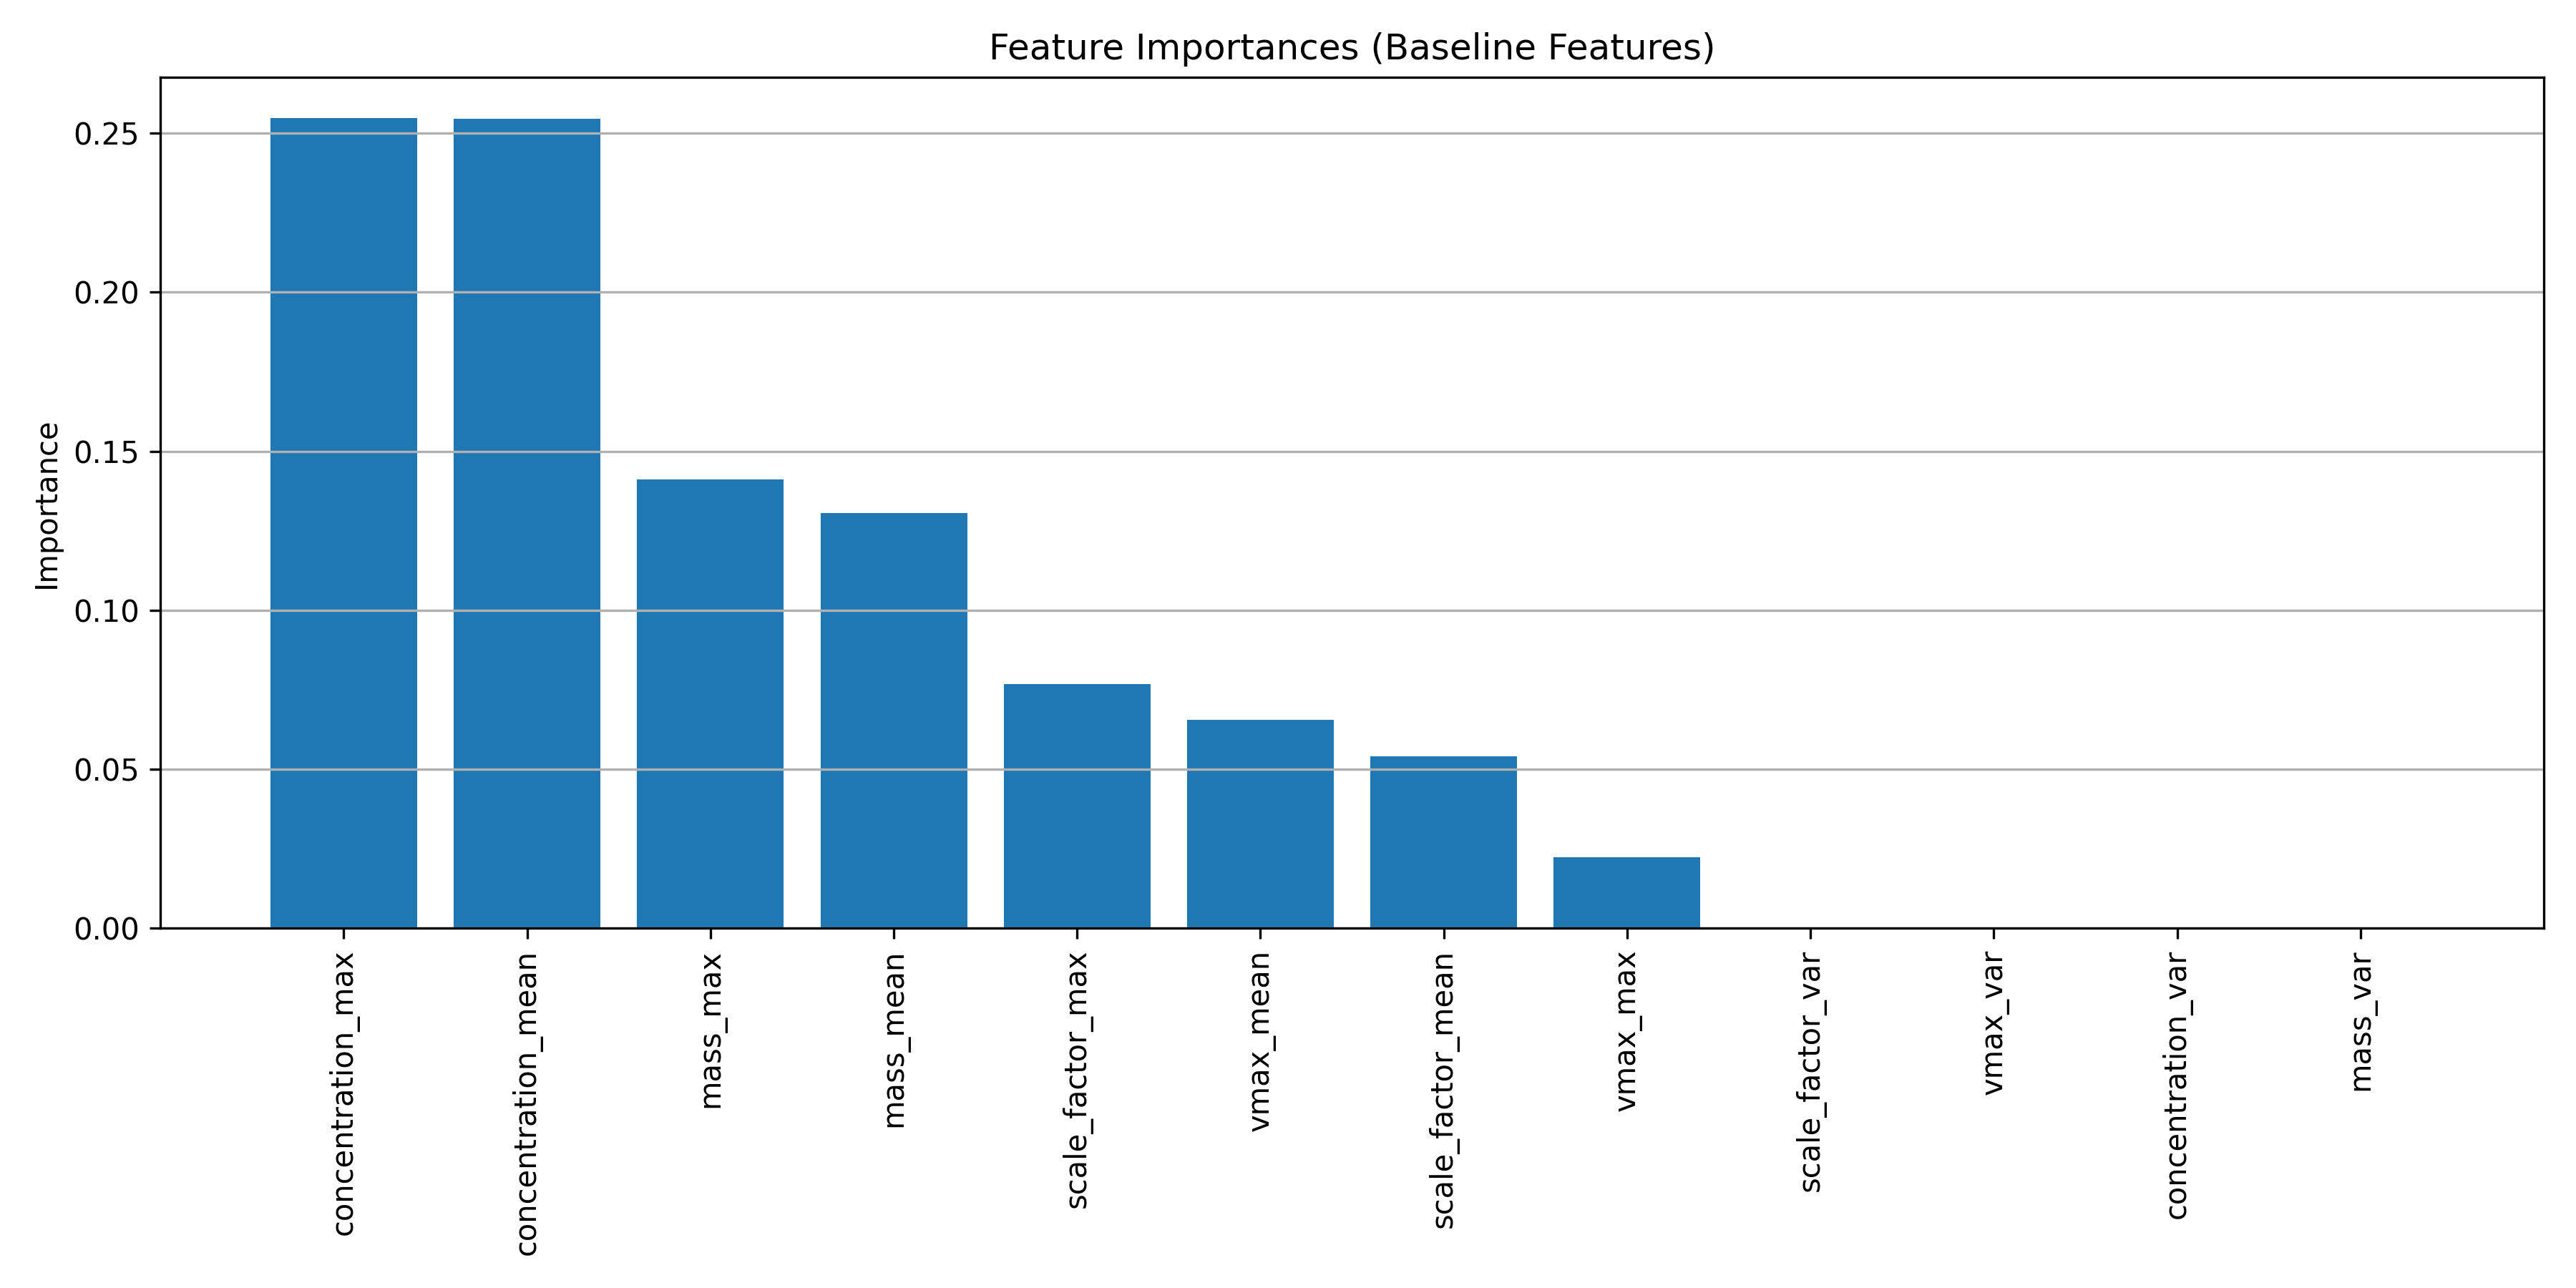
\includegraphics[width=0.5\textwidth]{../input_files/plots/feature_importances_baseline_3_20250524-175150.png}
    \caption{Feature importances for the baseline model, showing the relative importance of each feature in predicting final halo mass, though based on only N=5 samples.
}
    \label{fig:feature_importances_baseline}
\end{figure}

\begin{figure}[h!]
    \centering
    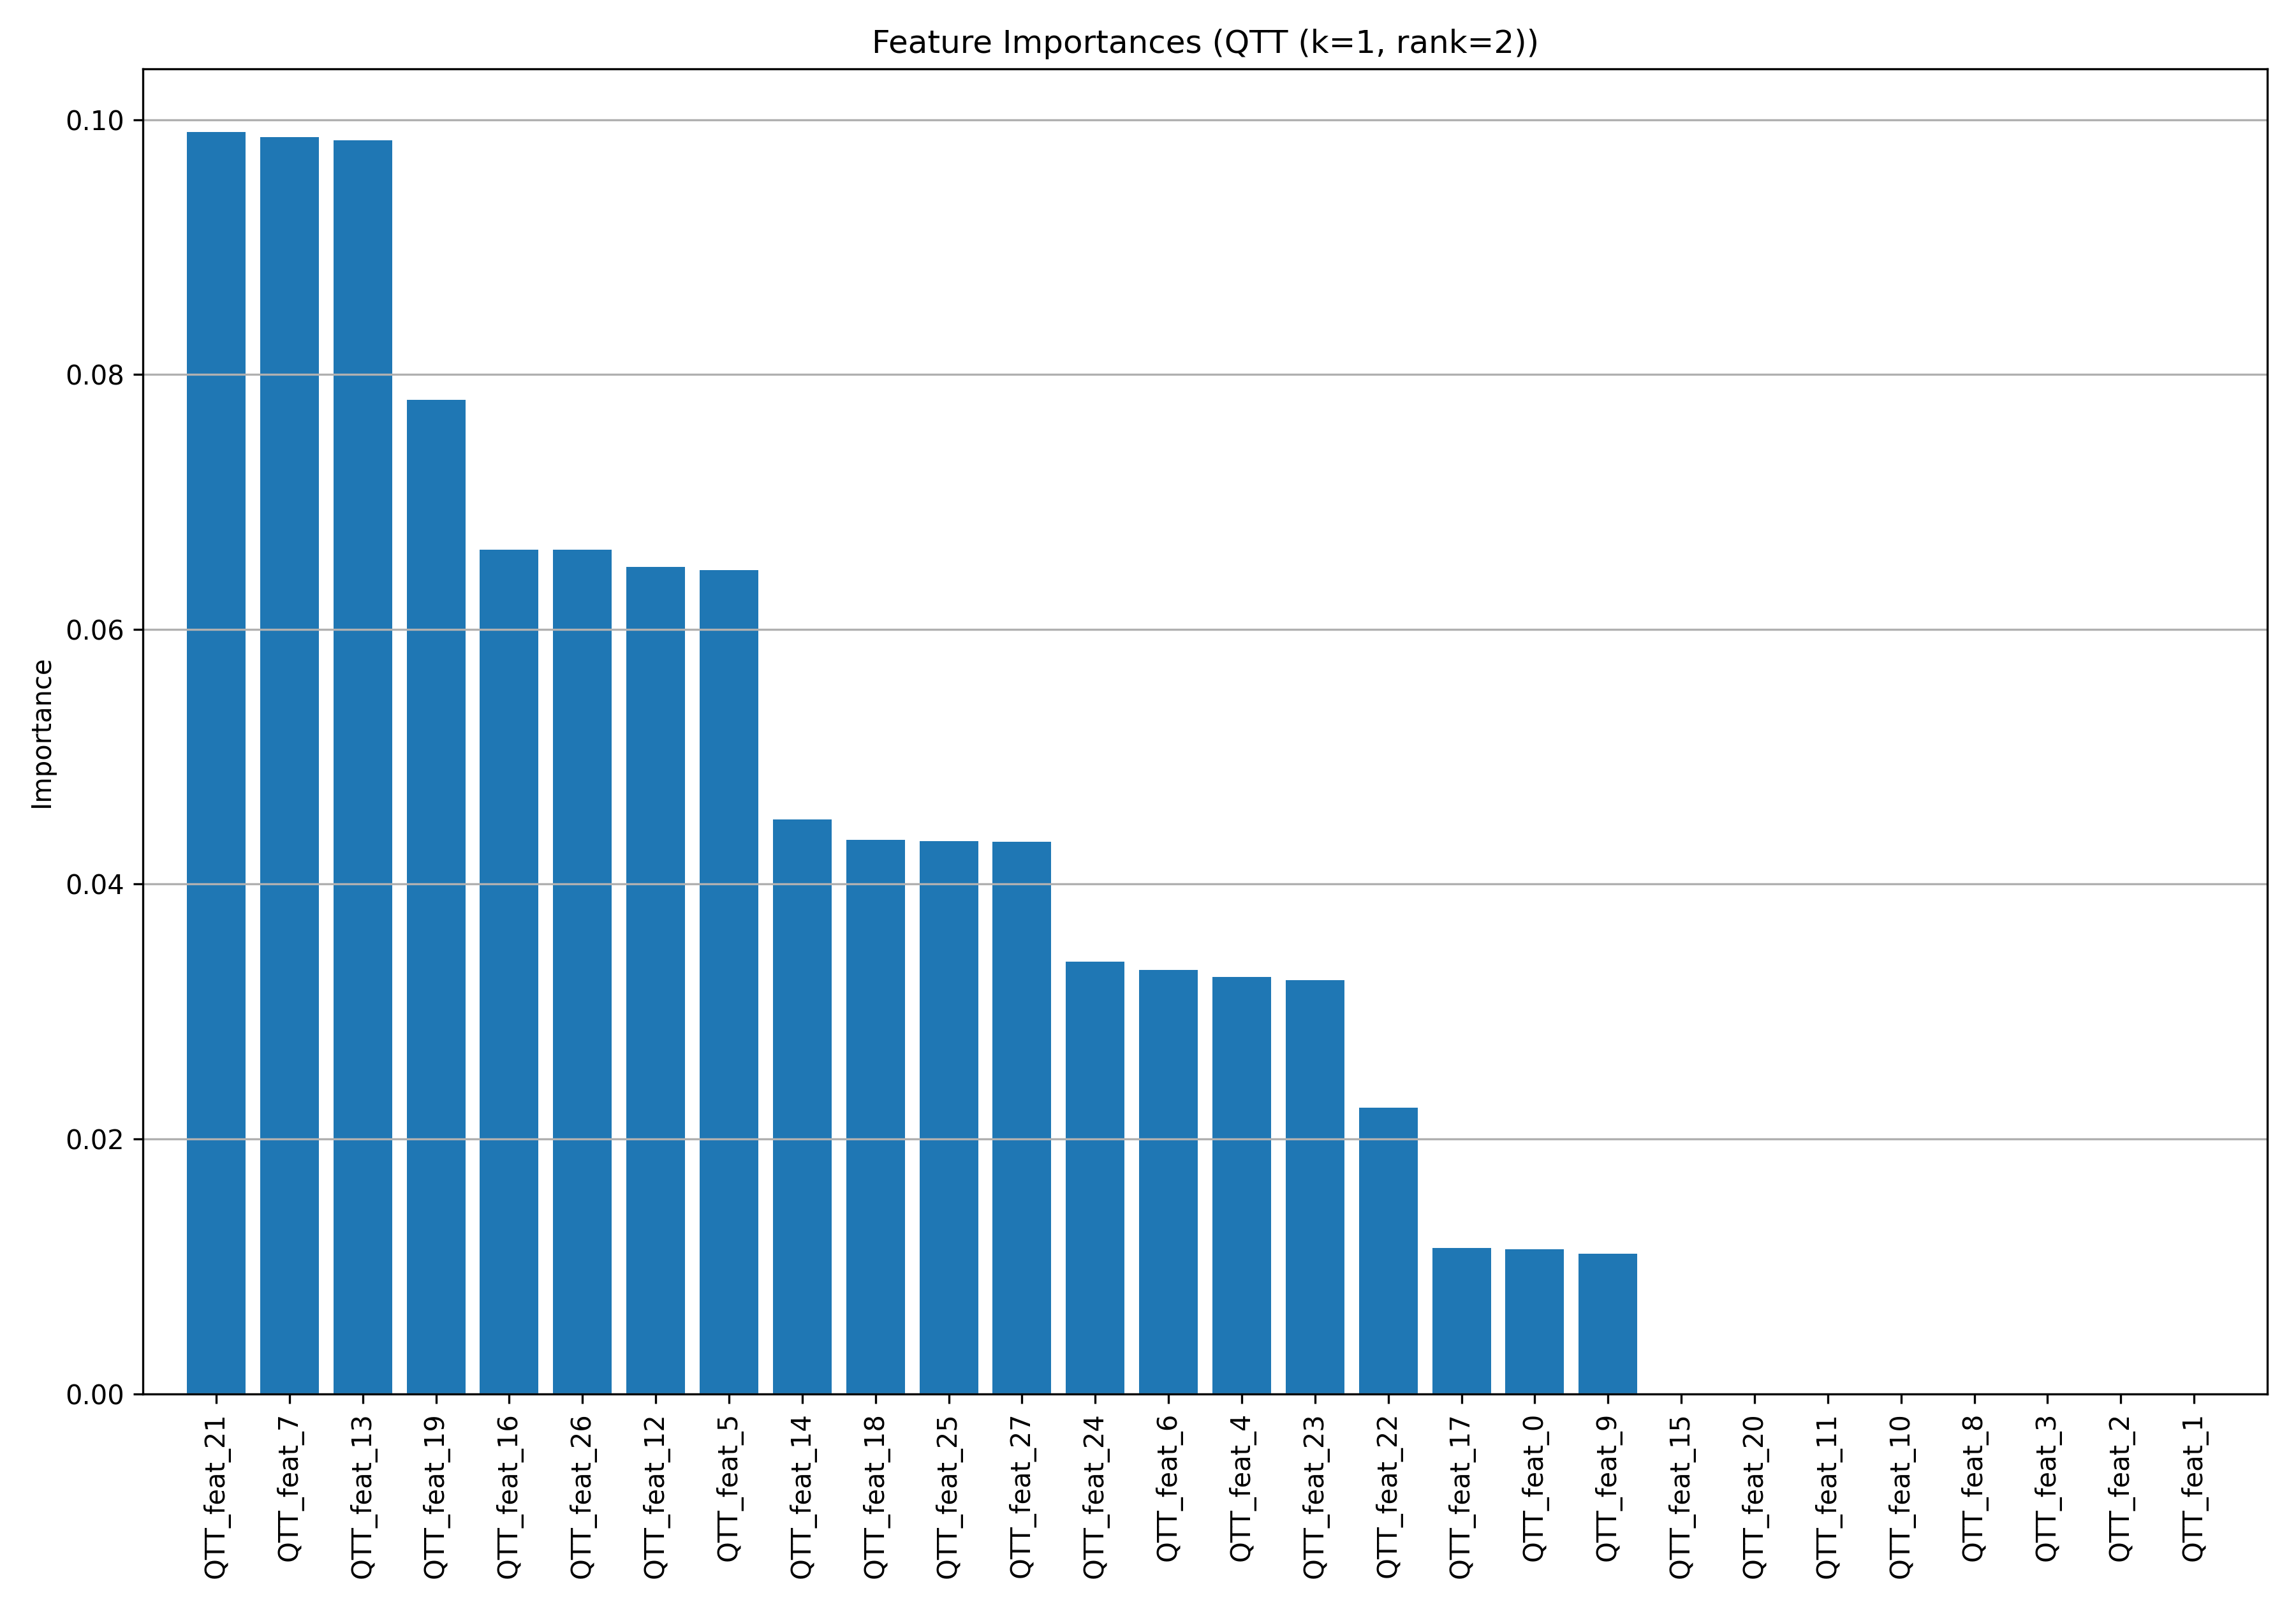
\includegraphics[width=0.5\textwidth]{../input_files/plots/feature_importances_qtt_k1_r2_6_20250524-175150.png}
    \caption{Feature importances derived from the Random Forest model trained on QTT features (k=1, rank=2) for predicting final halo mass, showing the relative contribution of each QTT feature. The varying importances suggest that different components of the compressed QTT representation contribute differently to the prediction task, although these importances are based on a limited sample size of N=5.
}
    \label{fig:feature_importances_qtt}
\end{figure}

\begin{figure}[h!]
    \centering
    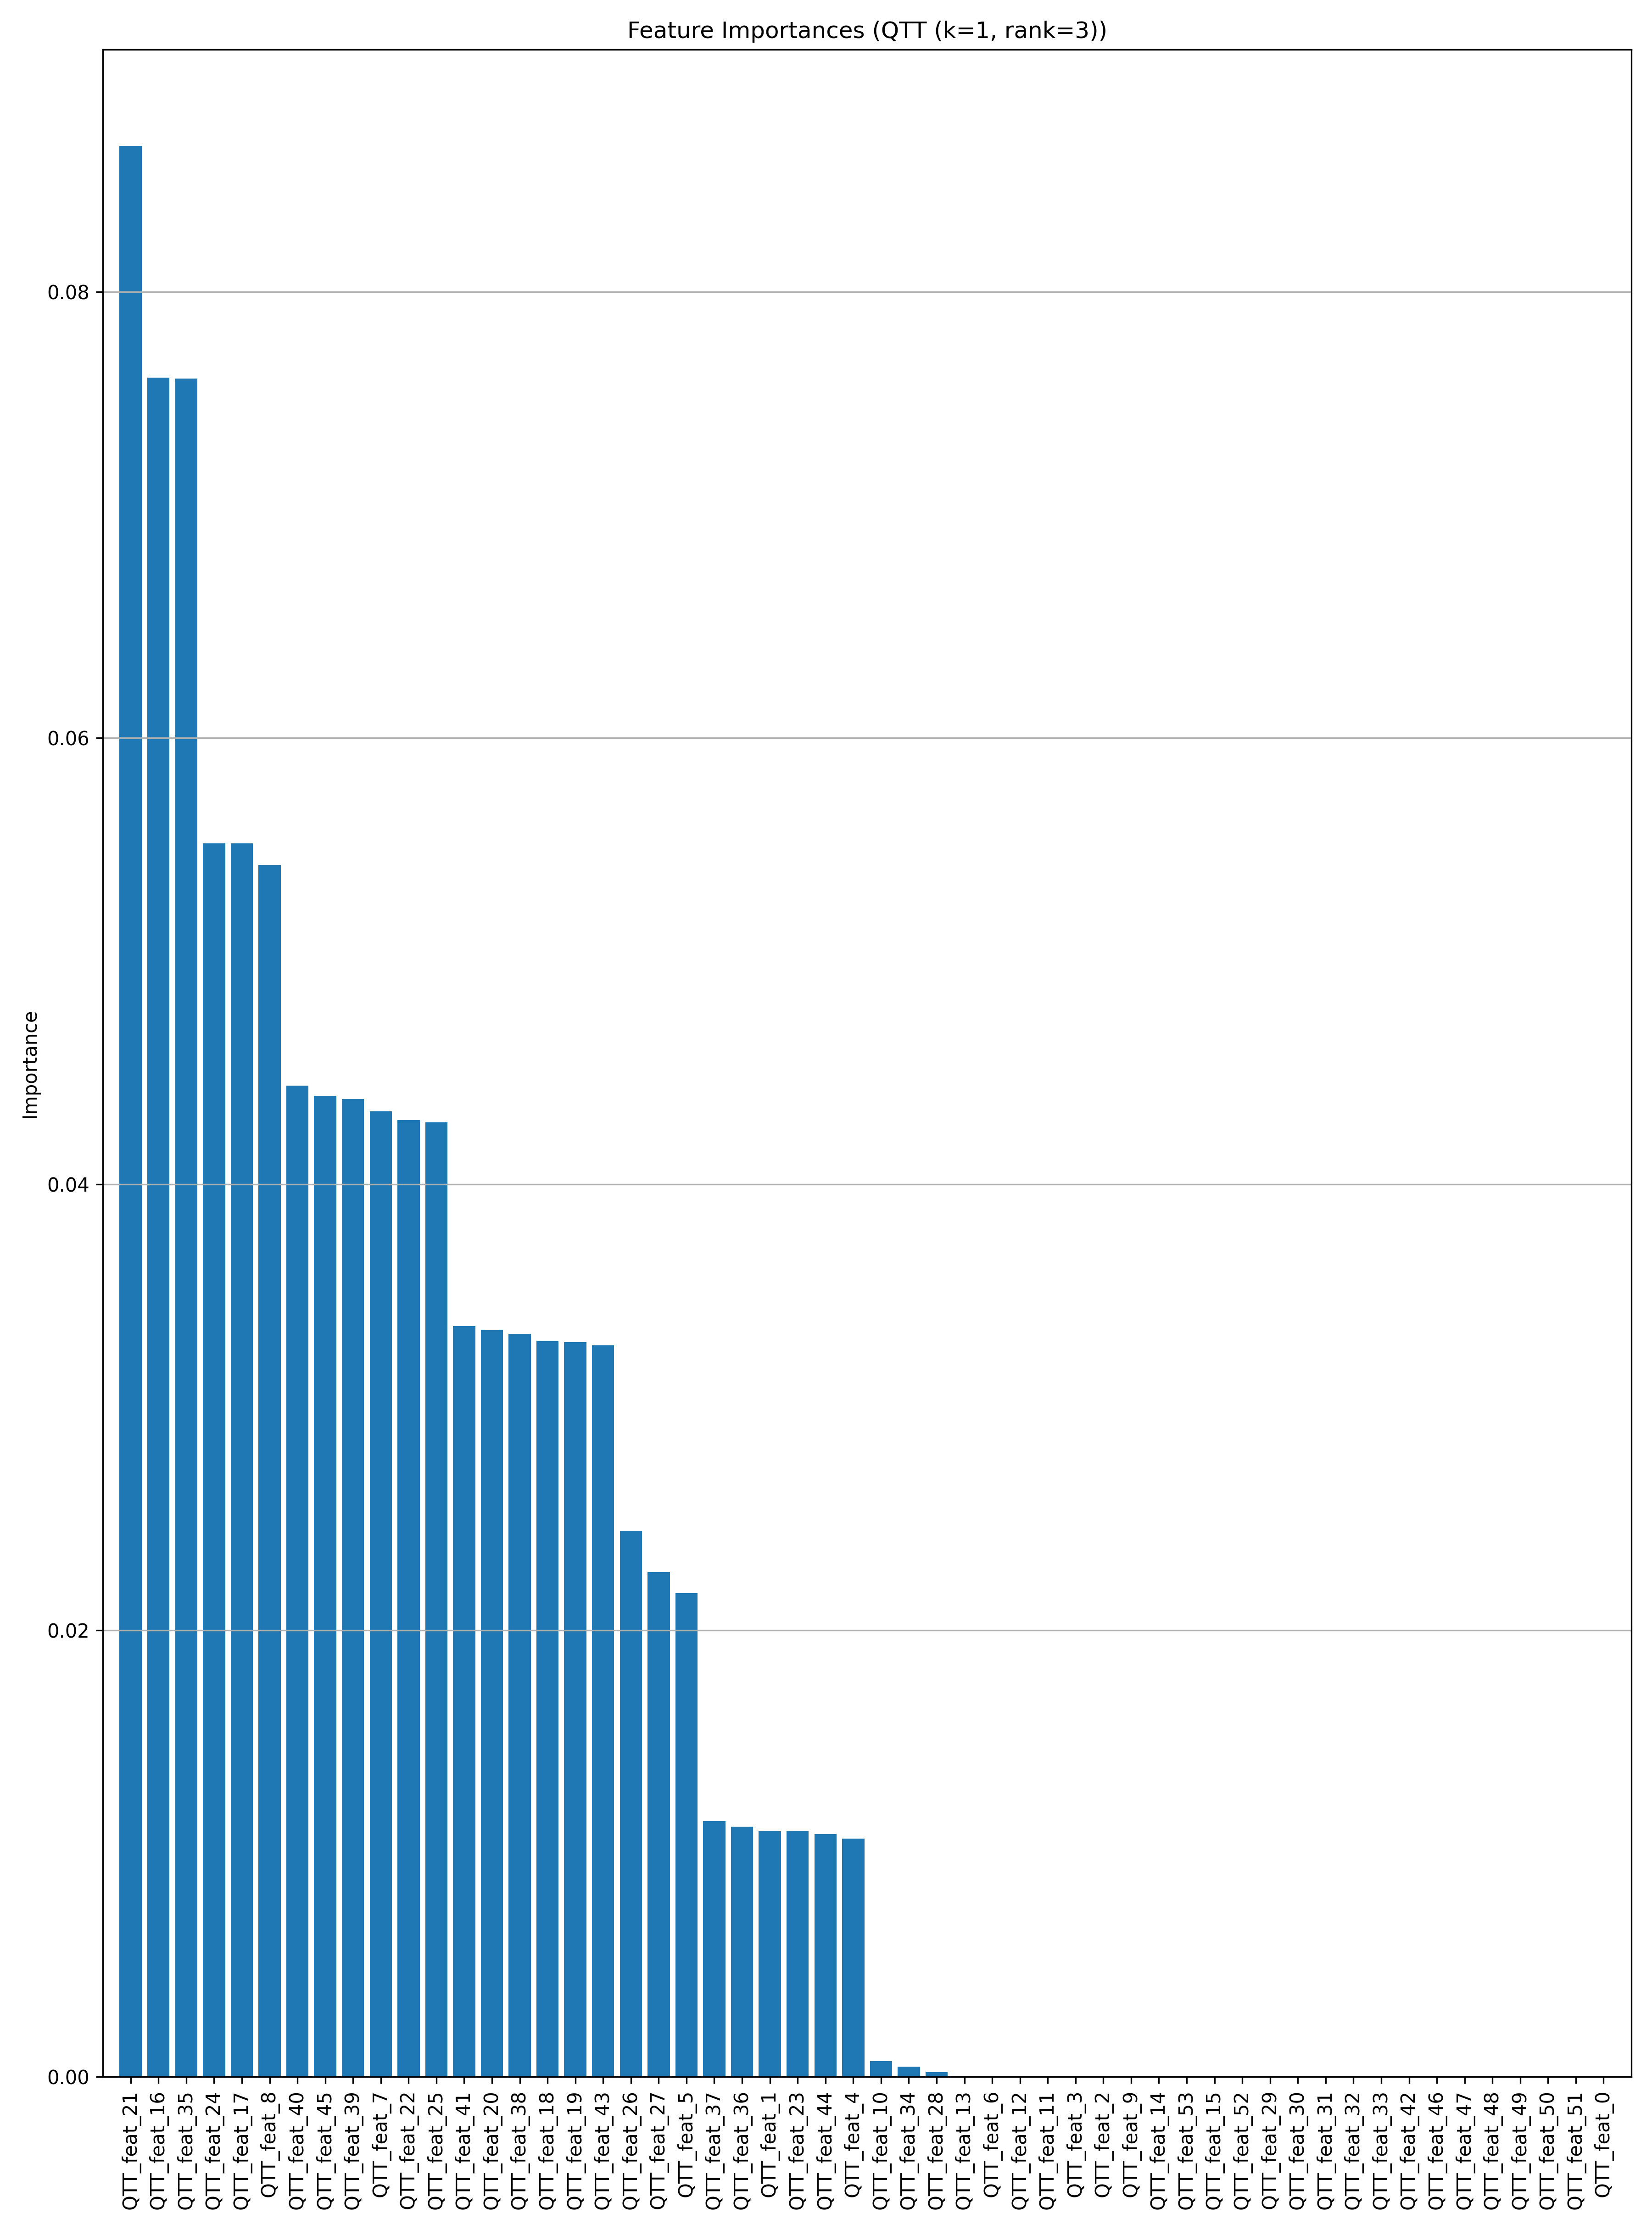
\includegraphics[width=0.5\textwidth]{../input_files/plots/feature_importances_qtt_k1_r3_9_20250524-175150.png}
    \caption{Feature importances for QTT features (k=1, rank=3) extracted from Random Forest models, showing the distribution of importances across the abstract QTT features. The varying importances suggest that different components of the compressed QTT representation contribute differently to the prediction task, although the small sample size (N=5) limits the generalizability of these observations.
}
    \label{fig:feature_importances_qtt_k1_r3}
\end{figure}

\begin{figure}[h!]
    \centering
    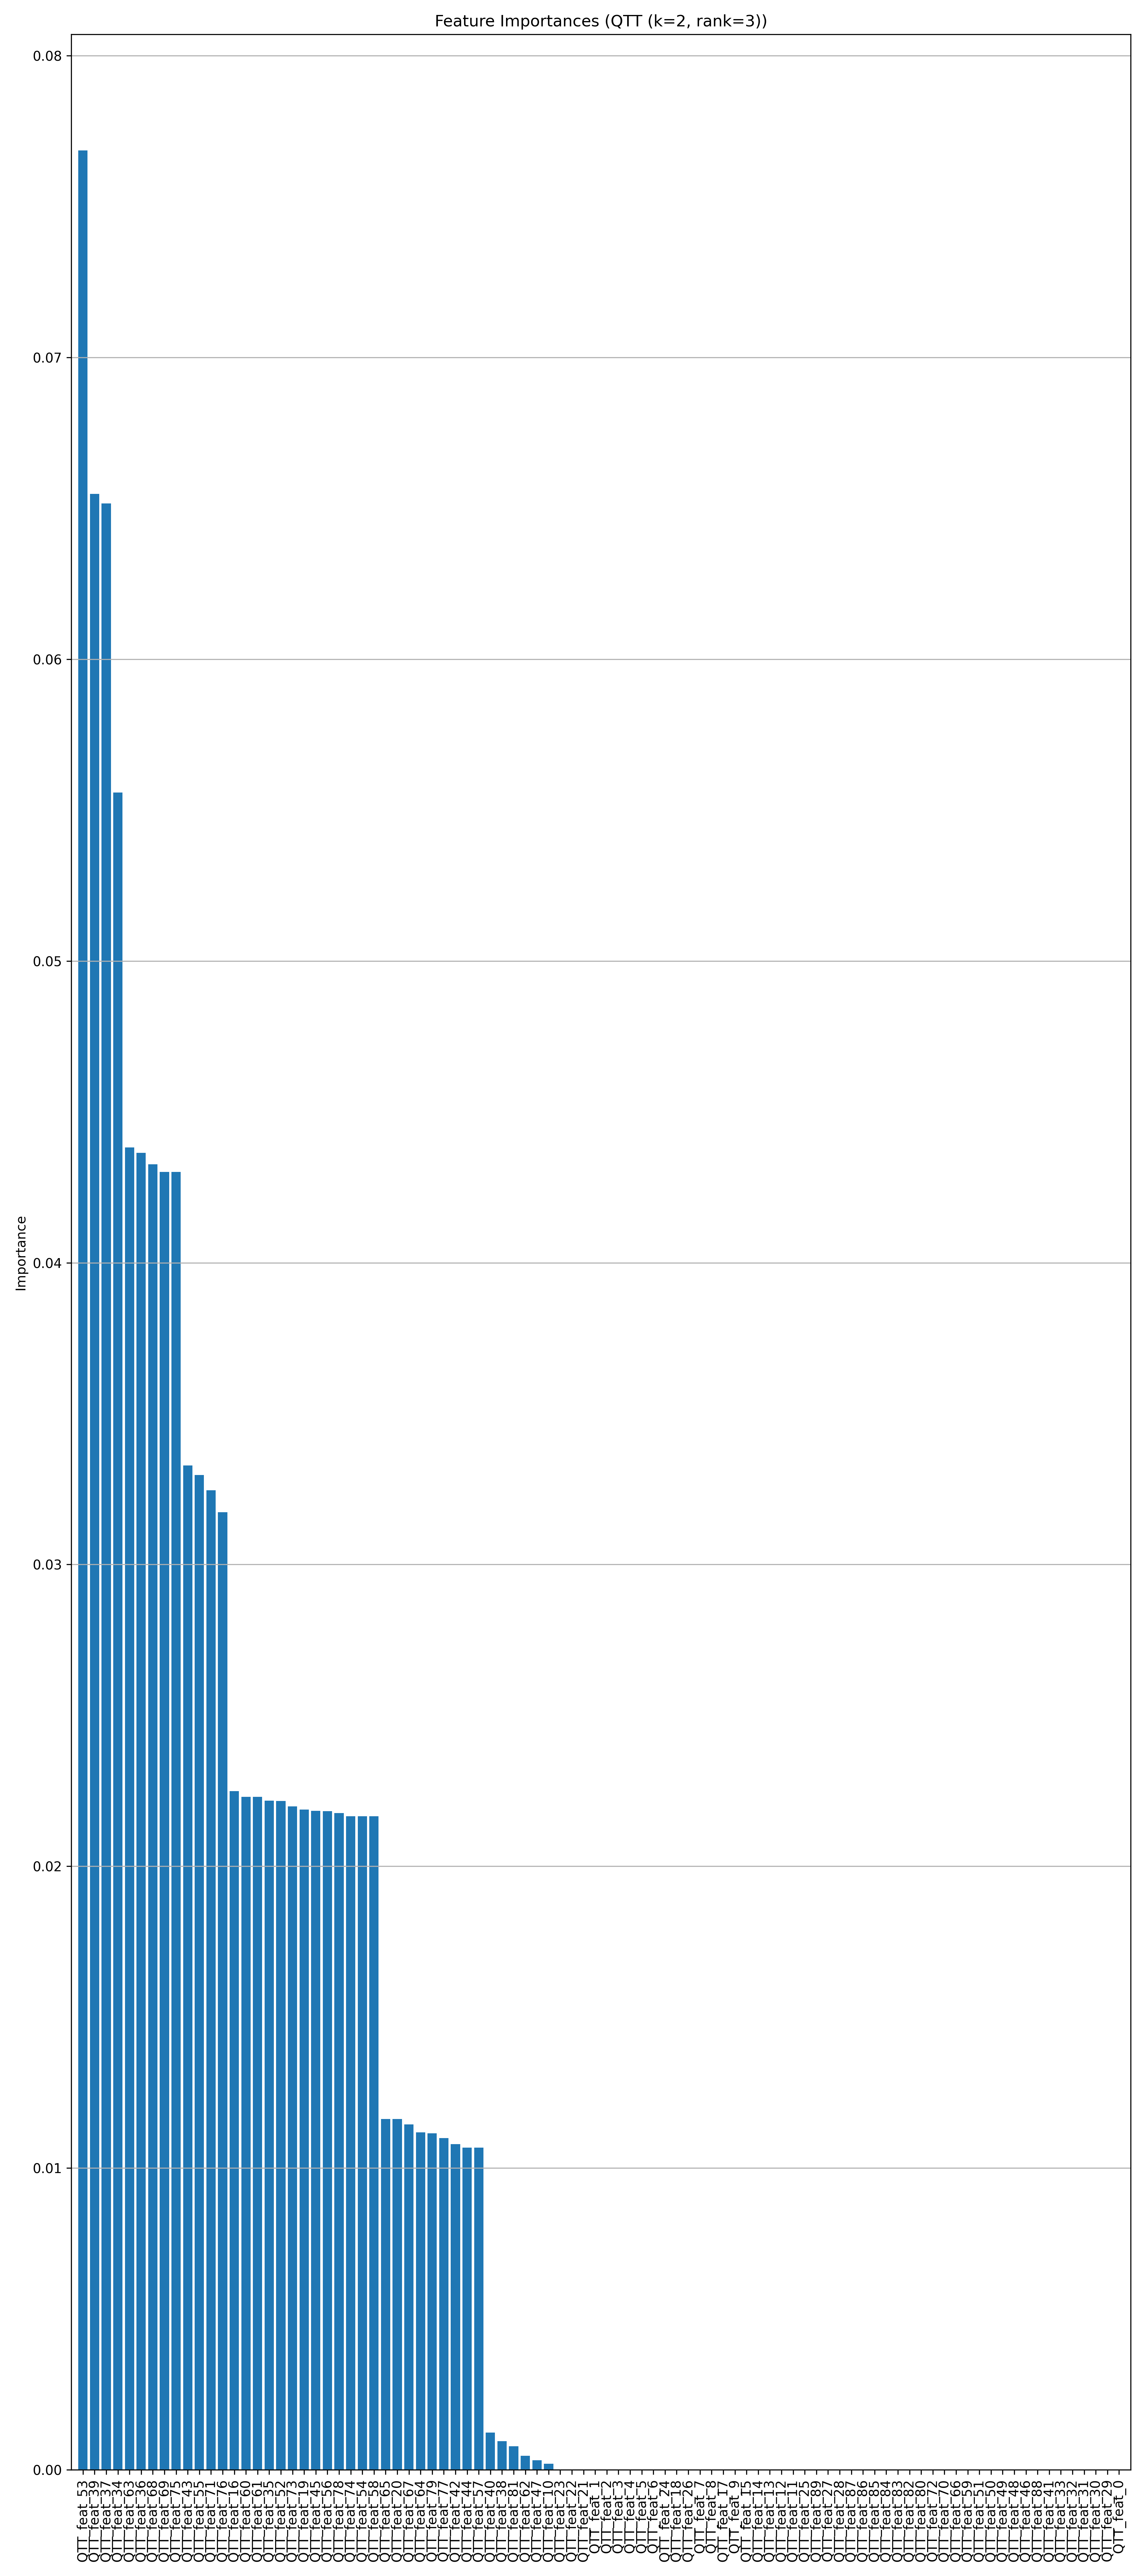
\includegraphics[width=0.5\textwidth]{../input_files/plots/feature_importances_qtt_k2_r3_15_20250524-175150.png}
    \caption{Feature importances derived from a Random Forest model trained on QTT features (k=2, rank=3). The importances reflect the contribution of each QTT feature to the prediction of final halo mass, though with only 5 samples, the individual feature importances are not robust.
}
    \label{fig:feature_importances_qtt_k2_r3}
\end{figure}

\begin{figure}[h!]
    \centering
    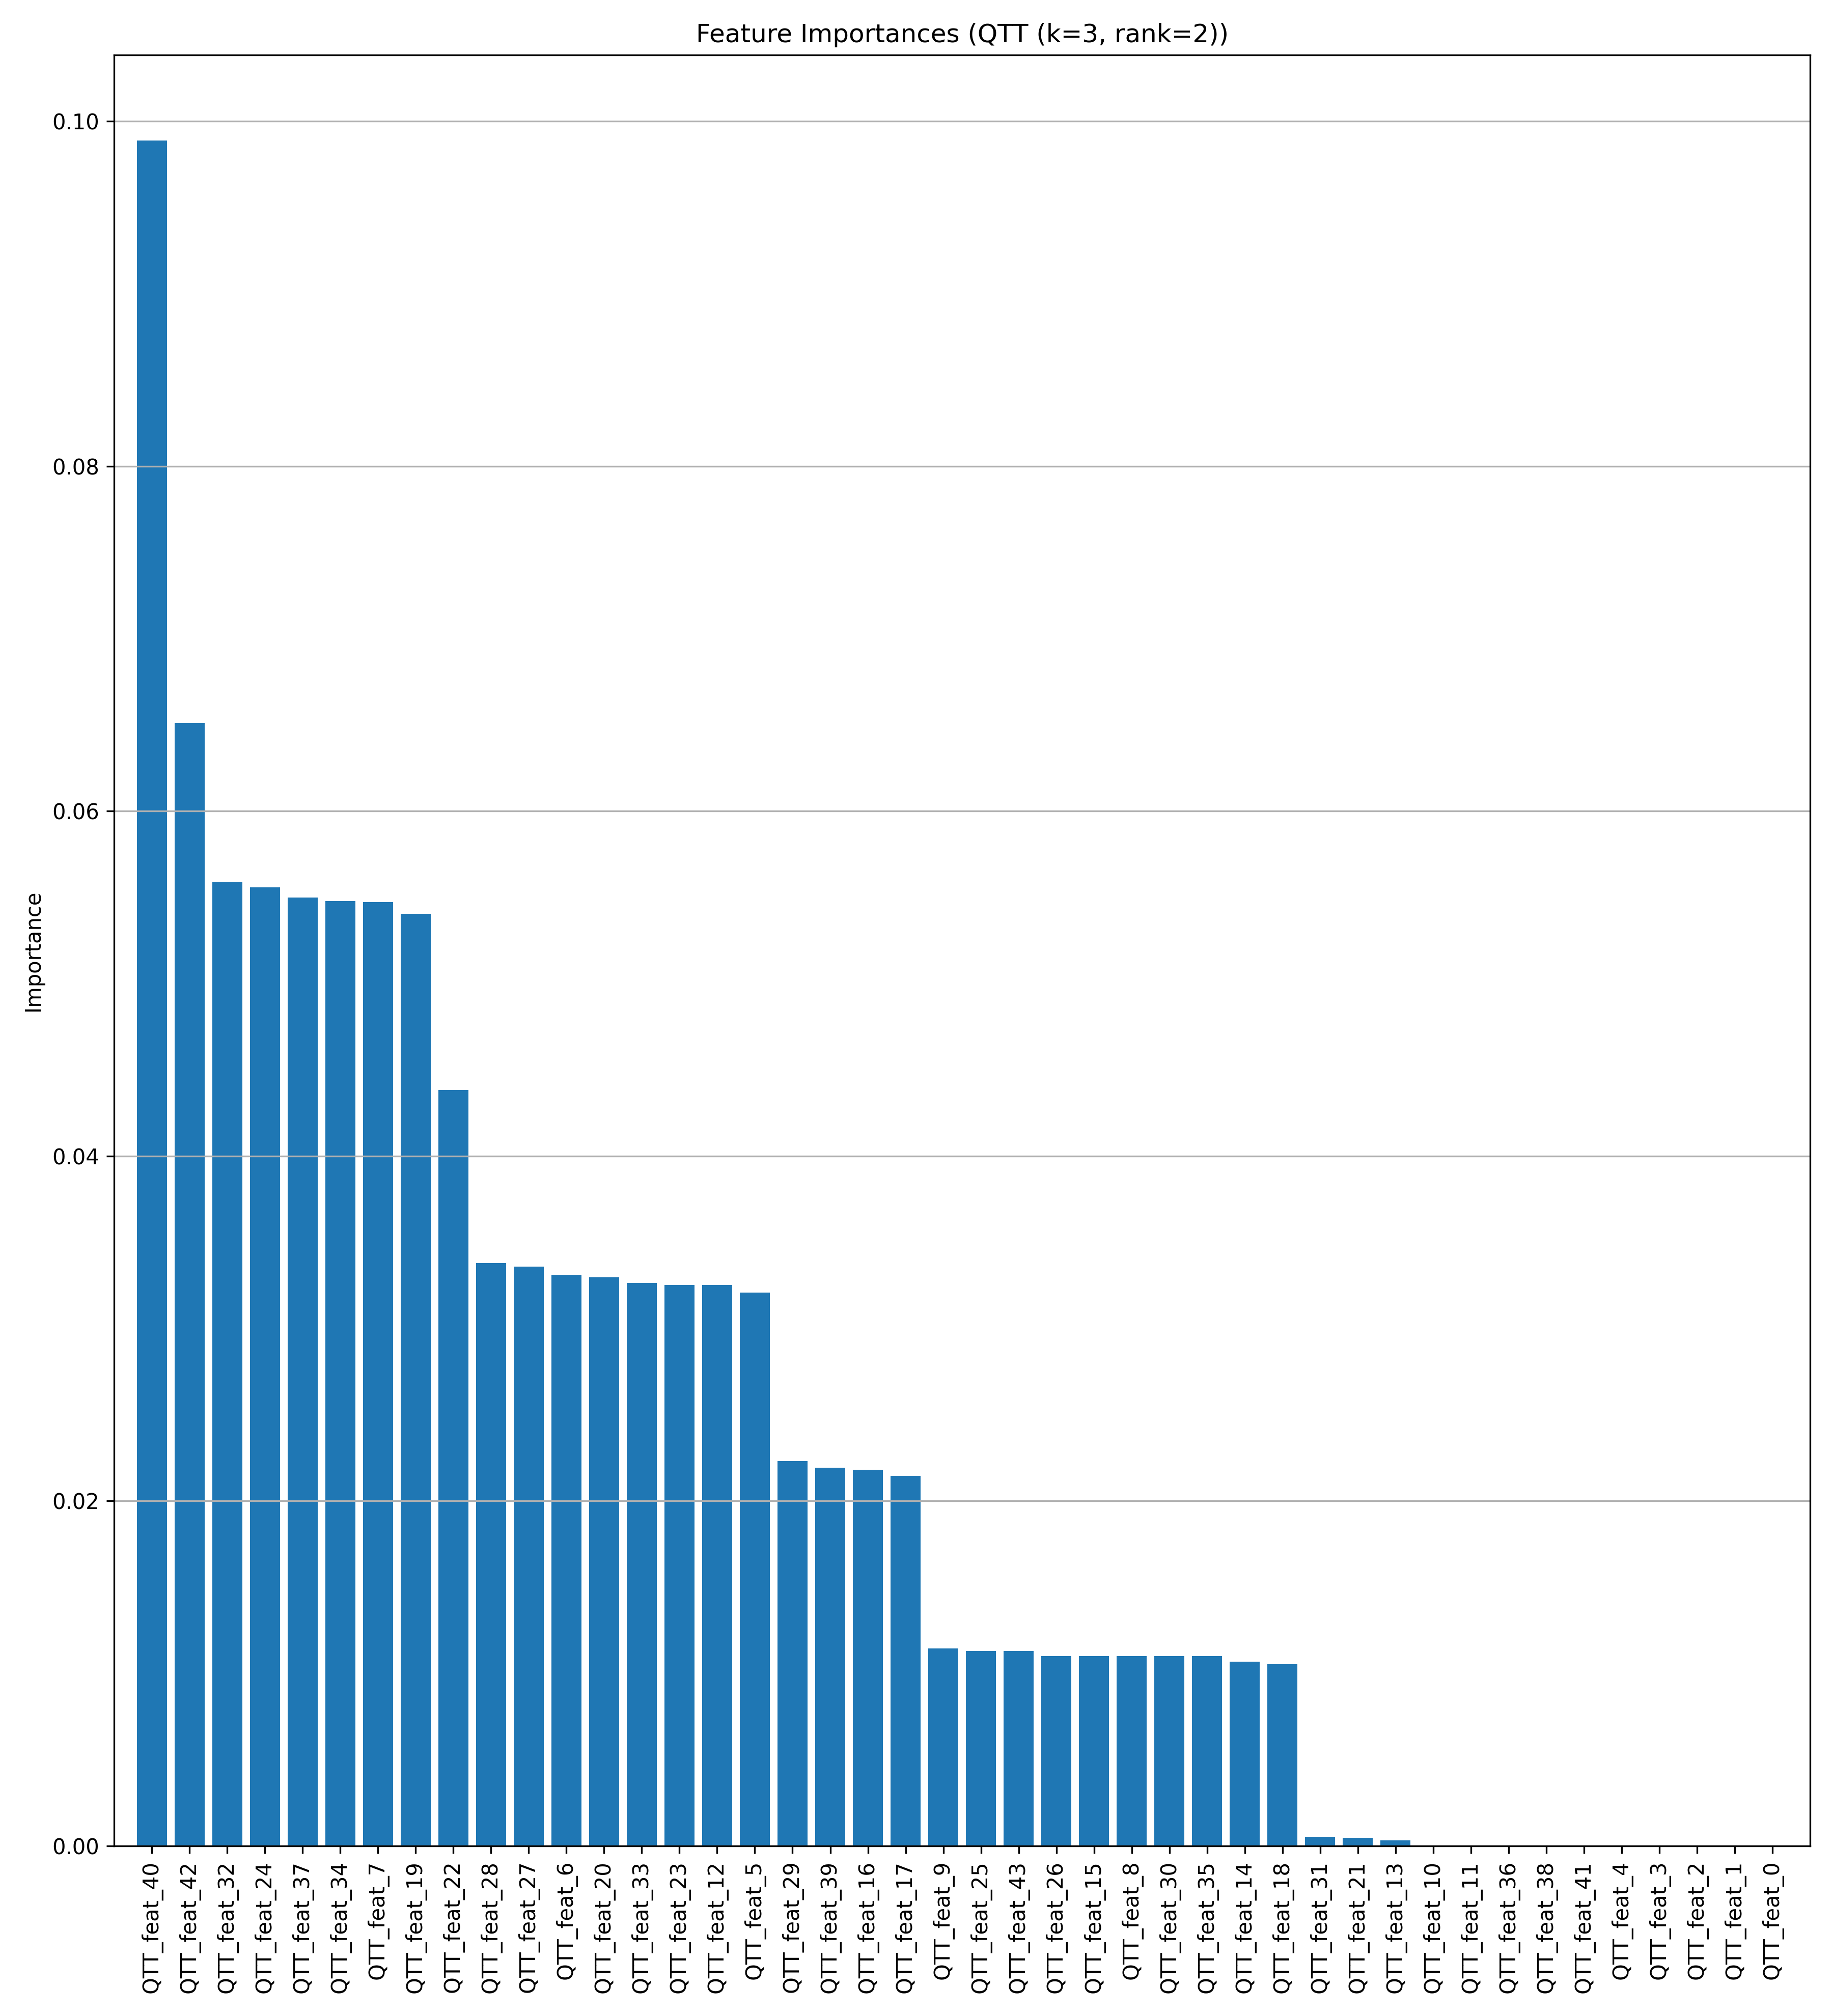
\includegraphics[width=0.5\textwidth]{../input_files/plots/feature_importances_qtt_k3_r2_18_20250524-175150.png}
    \caption{Feature importances derived from the random forest model trained on QTT features (k=3, rank=2) for predicting final halo mass, showing the varying contributions of individual QTT features despite their abstract nature and the limited sample size.
}
    \label{fig:feature_importances_qtt_k3_r2}
\end{figure}

\begin{figure}[h!]
    \centering
    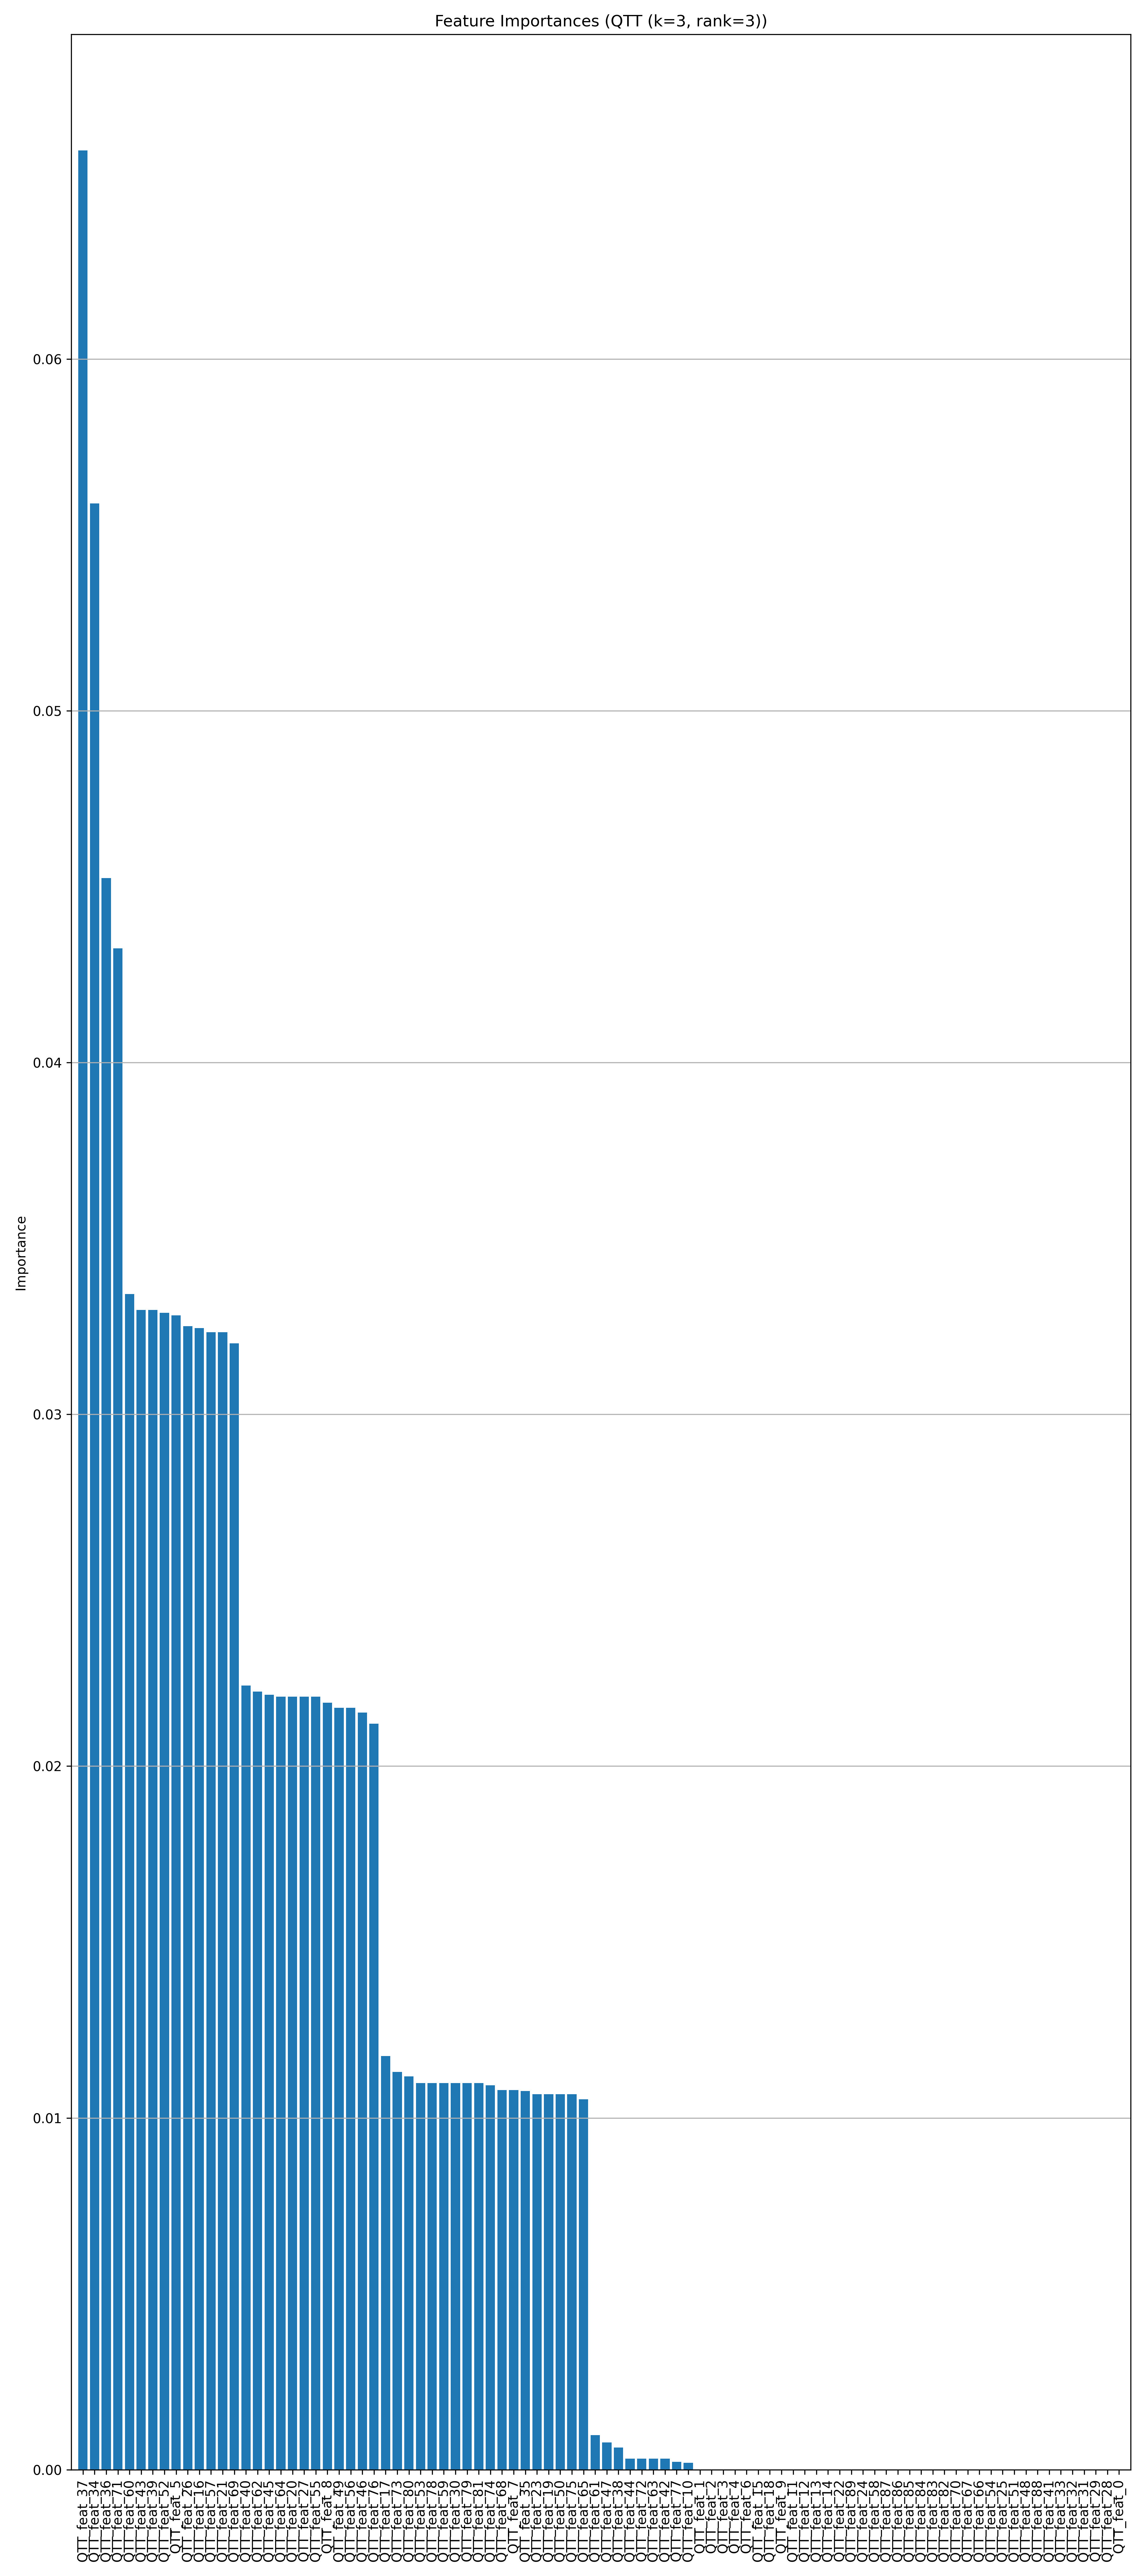
\includegraphics[width=0.5\textwidth]{../input_files/plots/feature_importances_qtt_k3_r3_21_20250524-175150.png}
    \caption{Feature importances derived from the Random Forest model trained on QTT features with $k=3$ and rank=3. While the model assigns varying importances to different QTT features, their abstract nature makes direct physical interpretation challenging given the small sample size.
}
    \label{fig:feature_importances_qtt_k3_r3}
\end{figure}

The utility of QTT features lies in their potential to automatically learn and encode complex, non-linear relationships and structural information from the local subgraph environment into a compact vector. This could be more powerful than simple statistical aggregations (mean, max, var) if the local graph structure and multi-feature interactions are important for the prediction task. However, this potential can only be validated with a much larger dataset.

\subsection{Impact of $k$-hop Neighborhood and QTT Rank}

Analyzing the table in Section 3.2:

\subsubsection{Impact of $k$}
For rank 2, performance (R²) decreased slightly as $k$ increased ($k=1$: 0.845, $k=2$: 0.834, $k=3$: 0.798). A similar, though less clear, trend is seen for rank 3. This might suggest that for this tiny dataset, larger subgraphs (larger $k$) introduced more noise or irrelevant information relative to the signal.

\subsubsection{Impact of QTT Rank}
Higher QTT rank allows for less compression and potentially captures more detail. However, this did not consistently translate to better predictive performance on this $N=5$ dataset. This could be due to overfitting with more complex features on such a small sample, or the specific information captured by the higher rank cores not being relevant for these 5 samples.

Again, these trends are based on $N=5$ and are not robust.

\subsection{Limitations and Future Directions Summary}

This study successfully implemented a pipeline for QTT-informed feature engineering on merger trees, demonstrating the feasibility of extracting and compressing information from local subgraph environments. Despite the promising reconstruction accuracy of QTT and the nominally high R² values achieved on the limited dataset, the core limitation lies in the extremely small effective sample size ($N=5$) due to issues with subgraph extraction. This prevents any meaningful conclusions regarding the generalizability or statistical significance of the results.

Future research should focus on resolving the subgraph extraction issue, validating the approach on larger datasets, exploring a wider range of QTT parameters, and comparing the performance against other methods like GNNs. Addressing these limitations will be crucial to realizing the full potential of QTT for feature engineering in cosmological merger tree analysis.

\end{document}
                